\documentclass[a4paper, twocolumn, 11pt, oneside]{memoir}
\usepackage{preamble}

% Path for graphics
\graphicspath{{./graphics/}}


\title{Rutherford Scattering}
\author[1]{Kirsten A. Juhl \thanks{201606487@post.au.dk}}
\author[1]{Henriette Ravn  \thanks{20116112@post.au.dk}}
\author[1]{Laurits N. Stokh olm \thanks{201605496@post.au.dk}}
\affil[1]{Department of Physics and Astronomy, Aarhus University}
\renewcommand{\Affilfont}{\itshape}
\date{\today}

% BibLateX

\usepackage[backend=biber, style=authortitle, defernumbers=true,
            sorting=nty]{biblatex}
            

\addbibresource{bibliography.bib}
\defbibheading{secbib}[\bibname]{%
    \section{#1}%
    \markboth{#1}{#1}}

%\raggedbottom
%\parindent = 0pt

%Følgende gør, at subscripts bliver ikke-kursiv. Anvendes X_|<subscript>|. Erstattes evt. med X_{\mathrm{<subscript>}}.
\makeatletter
\begingroup
\catcode`\_=\active
\protected\gdef_{\@ifnextchar|\subtextup\sb}
\endgroup
\def\subtextup|#1|{\sb{\textup{#1}}}
\AtBeginDocument{\catcode`\_=12 \mathcode`\_=32768 }
\makeatother

\DeclareSIUnit\gauss{G}

\begin{document}

% Dette er boksen i toppen. Lad den være.
%\vspace*{-13cm}
%\framebox[\textwidth][l]{\textbf{%
%\begin{tabular}{p{\linewidth}l}
%Received date: & {Approved:}\\
%& Date:\\
%& Signature:\\
%(reserved for instructor) & \\
%\end{tabular}
%}}
% Boksen slutter her .
%\vspace*{+1cm}
%\bigskip
% Title og Abstract
% Ignorerer twocolumn til abstract
\begin{minipage}{\textwidth}
    \twocolumn[
        \maketitle
        \begin{onecolabstract}
        \noindent
            This paper is written as the \emph{first} of four mandatory repports
during the course \emph{Experimental Physics III}.

In the experiment we will be working with ... 

At last ....


This resulted in ...
in confirmation of the theory

        \end{onecolabstract}]
\end{minipage}
\saythanks{}
%\vspace{9cm}
\section{Introduction} 
Almost all of our knowledge in the field of nuclear and atomic physics has been discovered through scattering experiments,and the theory of scattering underpins one of the most ubiquitous tools in physics.
In low energy physics, scattering phenomena provide the standard tool to
explore solid state systems. Historically, this was used as a first step
towards our current understanding of the atom.

This paper examines the Rutherford scattering of a beam of $\SI{350}{\kilo\electronvolt}$ protons on a thin foil of $\mathrm{Au}$/$\mathrm{C}$ target. To limit the extend of the paper, and to keep our discussion simple and relevant, we will only examine elastic collisions in the semi-classical regime, governed by the Sommerfeld criterion for classical scattering. \cite[p. 14]{noteBB}

This is usually fine for low energy physics, in which internal energies remain
constant and no further particles are created or annihilated.
For this experiment, which uses a single Van-de-Graaff accelerator to generate particles with energies of up to $\SI{400}{\kilo\electronvolt}$, this is a good approximation.

%\vfill



%\section{Theory}

%\section{Hazards}
This experiment has primarily $3$ major hazards to be aware of, as listed below

\begin{itemize}
    \item High Voltage (HV). High severity, low risk. Turn off the power, and
        let it cool before switching it off on the O/I button. Especial care,
        if wearing a pacemaker or the alike.
    \item Lead poisoning. Low Severity, low risk. Do not touch the lead blocks.
        If necessary, use glows and wash hands. Do not eat or drink in the
        laboratory.
    \item Radioactivity. Low severity, low risk. Be careful when handling the
        radiation sources. Do not eat or drink in the laboratory. 
\end{itemize}

\section{Materials and Methods}
\subsection{Experimental Setup}
To obtain energies in the order of a $\SI{400}{\kilo\electronvolt}$, a single Van-de-Graaf
accelerator (see \cref{fig_setup3}) was used. The variety of incomming beam particles
was limited by the source (a flask of hydrogen gas connected to the accelerator
tank). Therefore, we only concider incomming ions $\mathrm{H^+}$ and
$\mathrm{{H_{2}}^{+}}$, as the source was stationary, and not changed.
%
\begin{figure}[t]
    \centering
    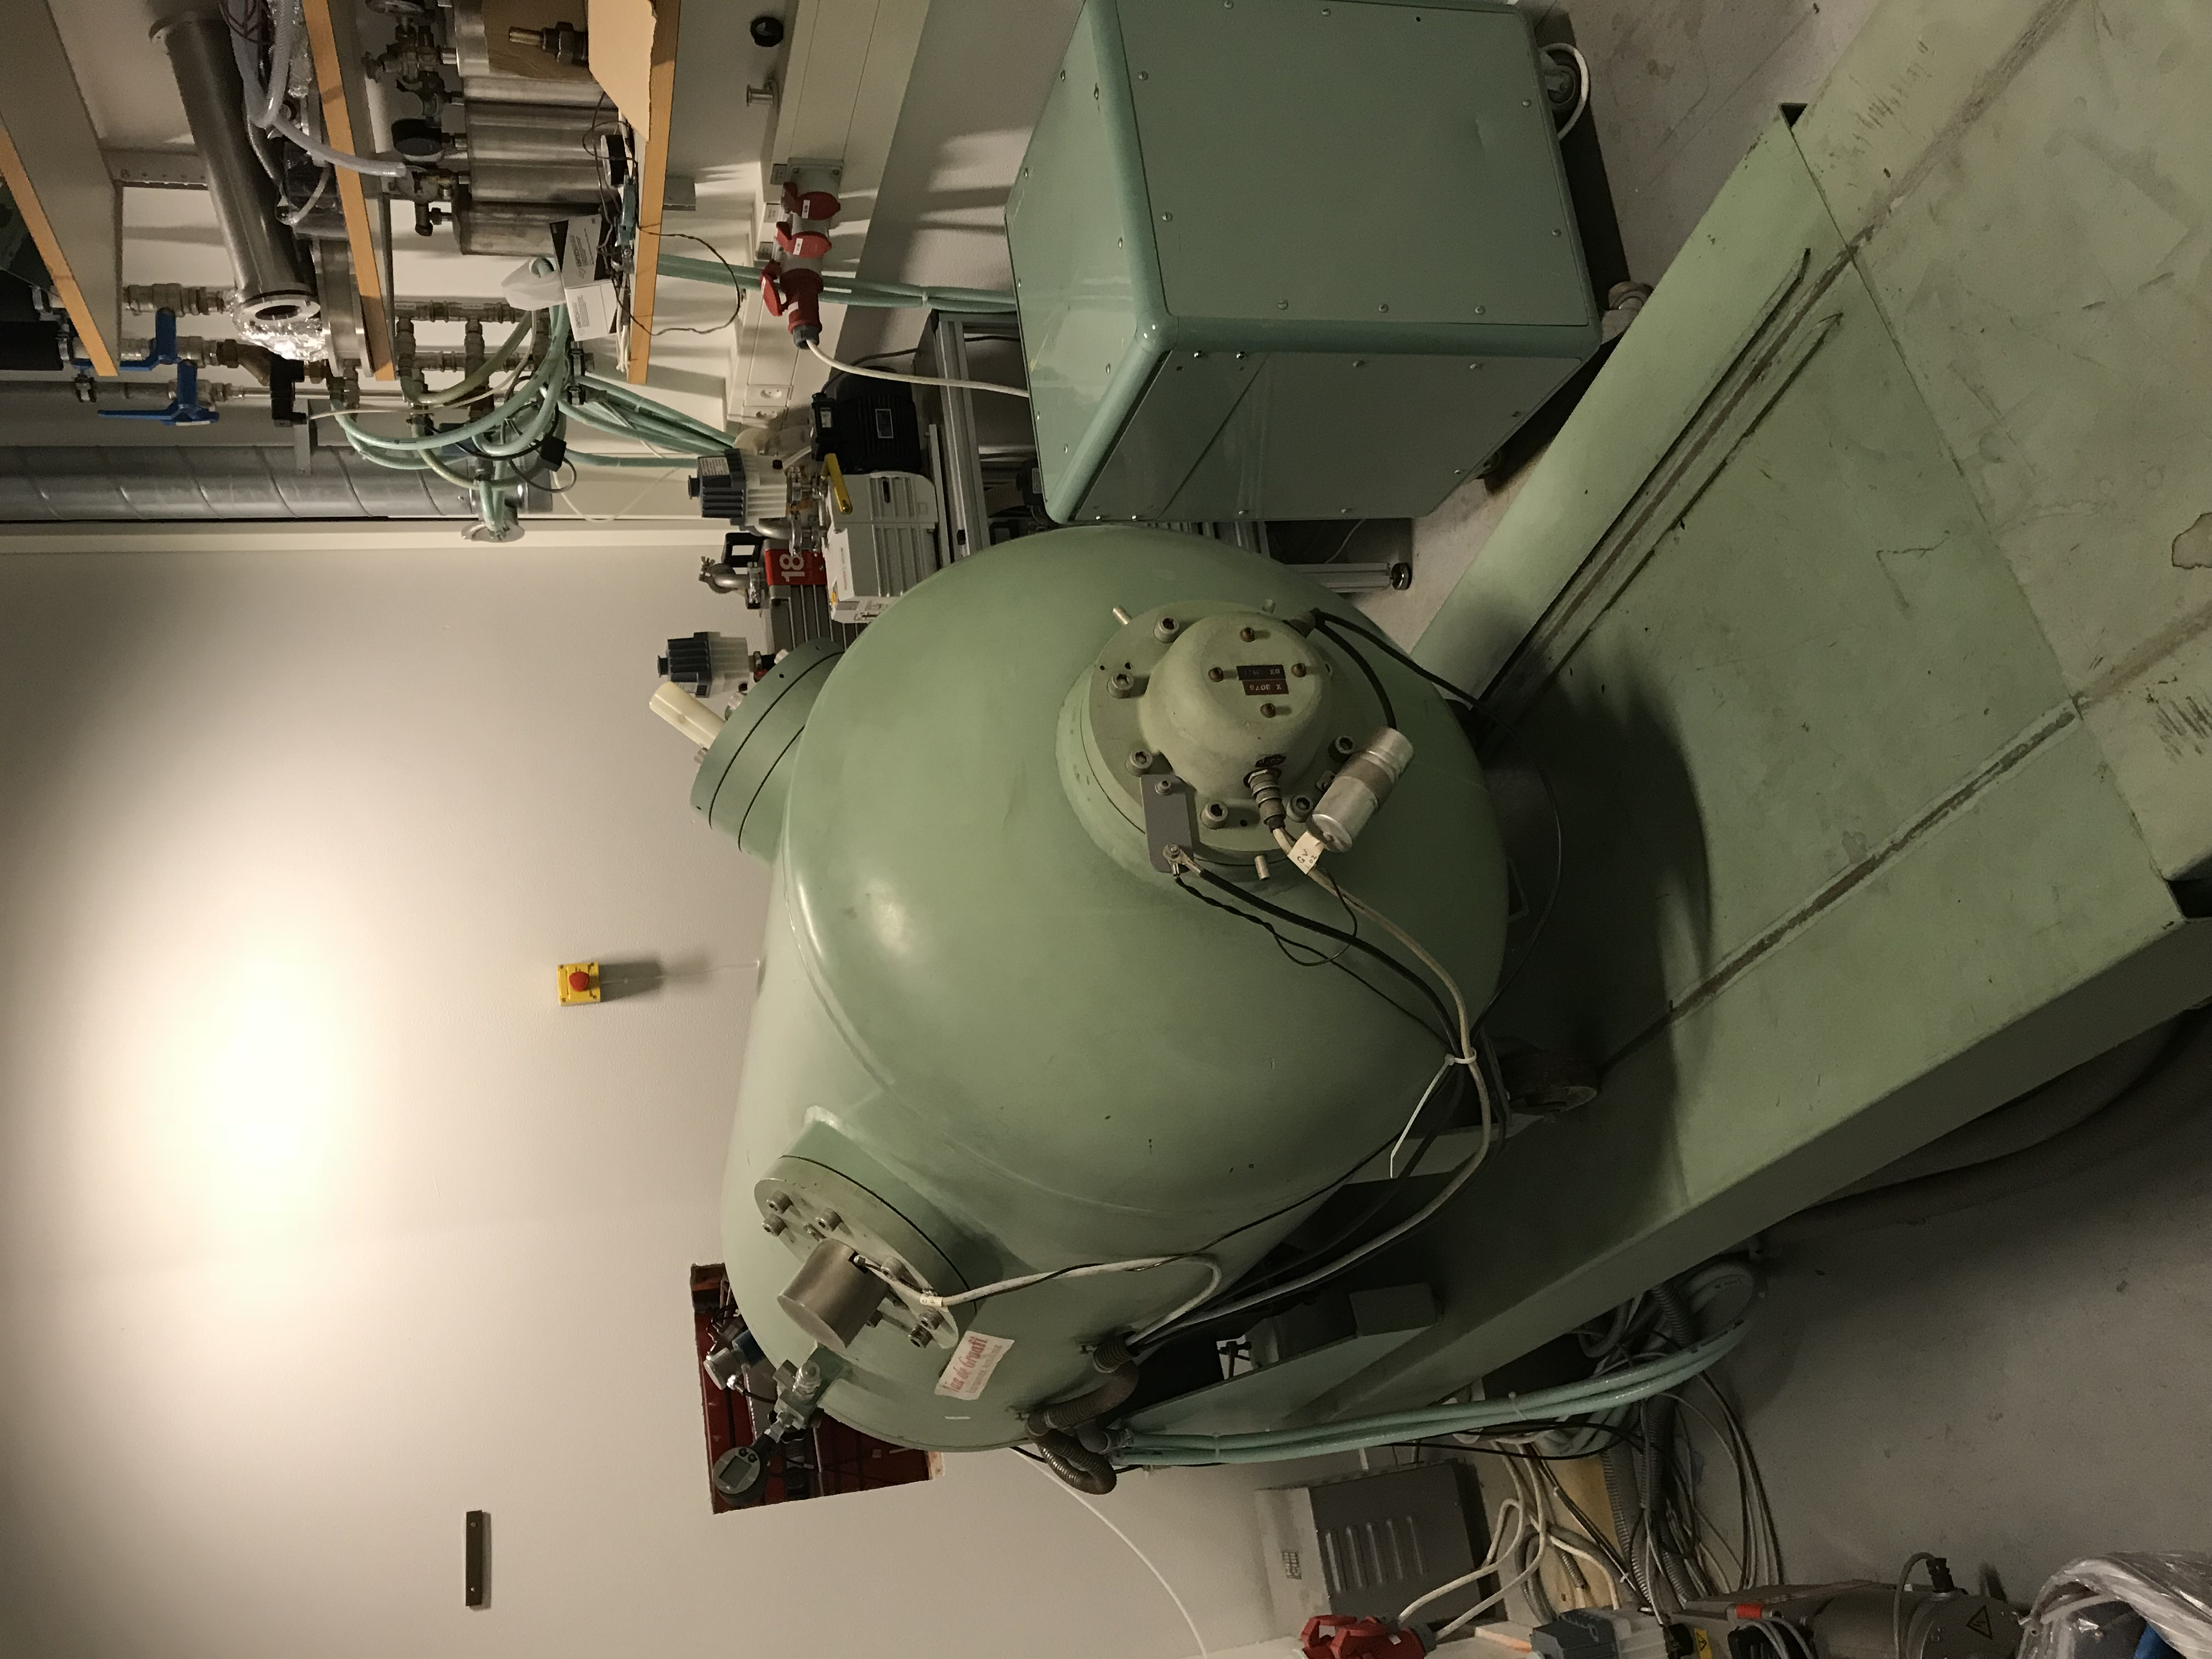
\includegraphics[angle=-90, trim={35cm, 0cm, 27cm, 0cm}, clip,  width=0.99\columnwidth]{setup3}
    \caption{The Van-de-Graaf accelerator.}
    \label{fig_setup3}
\end{figure}
%
Acceleration of the ions was controllable by changing the voltage drop on the
dashboard (see \cref{fig_setup2}), and thus also the kinetic energy of the
incomming beam. This will be described furhter in the section Procedure.

The detector was at an angle of the accelerator arm, and by changing the
magnetic field strength of the electromagnet, one can choose which of the two
possible incomming ions was deflected to interact with the target.
The motion of a charged particle in a magnetic field is governed by the Lorentz
force law, and as the trajectory of the motion is traced as part of a circle,
one obtains the necesarry equality for the motion to be\footnote{Dealing with
    forces and spatial confinements to circular paths is true in the classical
    regime. Had we wanted a fully relativistic and quantum mechanical
description, this would not be the case.}
\begin{equation}
F_|m| = QvB = F_|cp| = \frac{mv^2}{r}.
\end{equation}
This gives a ratio of the two magnetic fields needed for the respective ions
\begin{align}
    R_|B| = & \frac{B({H_2}^+)}{B(H^+)} = \frac{m({H_2}^+)
    v({H_2}^+)}{m(H^+)v(H^+)}\\
    & 2 \frac{v({H_2}^+)}{v(H^+)} = \sqrt{2}
\end{align}
%
By assuming that the mass of the two ions are related by $m(H^+) =
2m({H_2}^+)$, and using $v(X) = \sqrt{\frac{2E}{m(X)}}$ for each ion.
%
Given one of the magnetic fields, the other is determined by this ratio factor.
We used the following magnetic fields for the two ions:
%
\begin{equation}
    B(H^+) = \SI{1070}{\gauss} \quad B({H_2}^+) = \SI{1513}{\gauss}
\label{}
\end{equation}
%
Conclusively, by changing the magnetic field strength, one changes the
incomming ion. BE AWARE: The magnetic field can change over the time scale of meassurements
due to mechanical heating of the metal in the electromagnet. This leads to expansion and thus
the magnetic field will be reduced.
%
\begin{figure}[t]
    \centering
    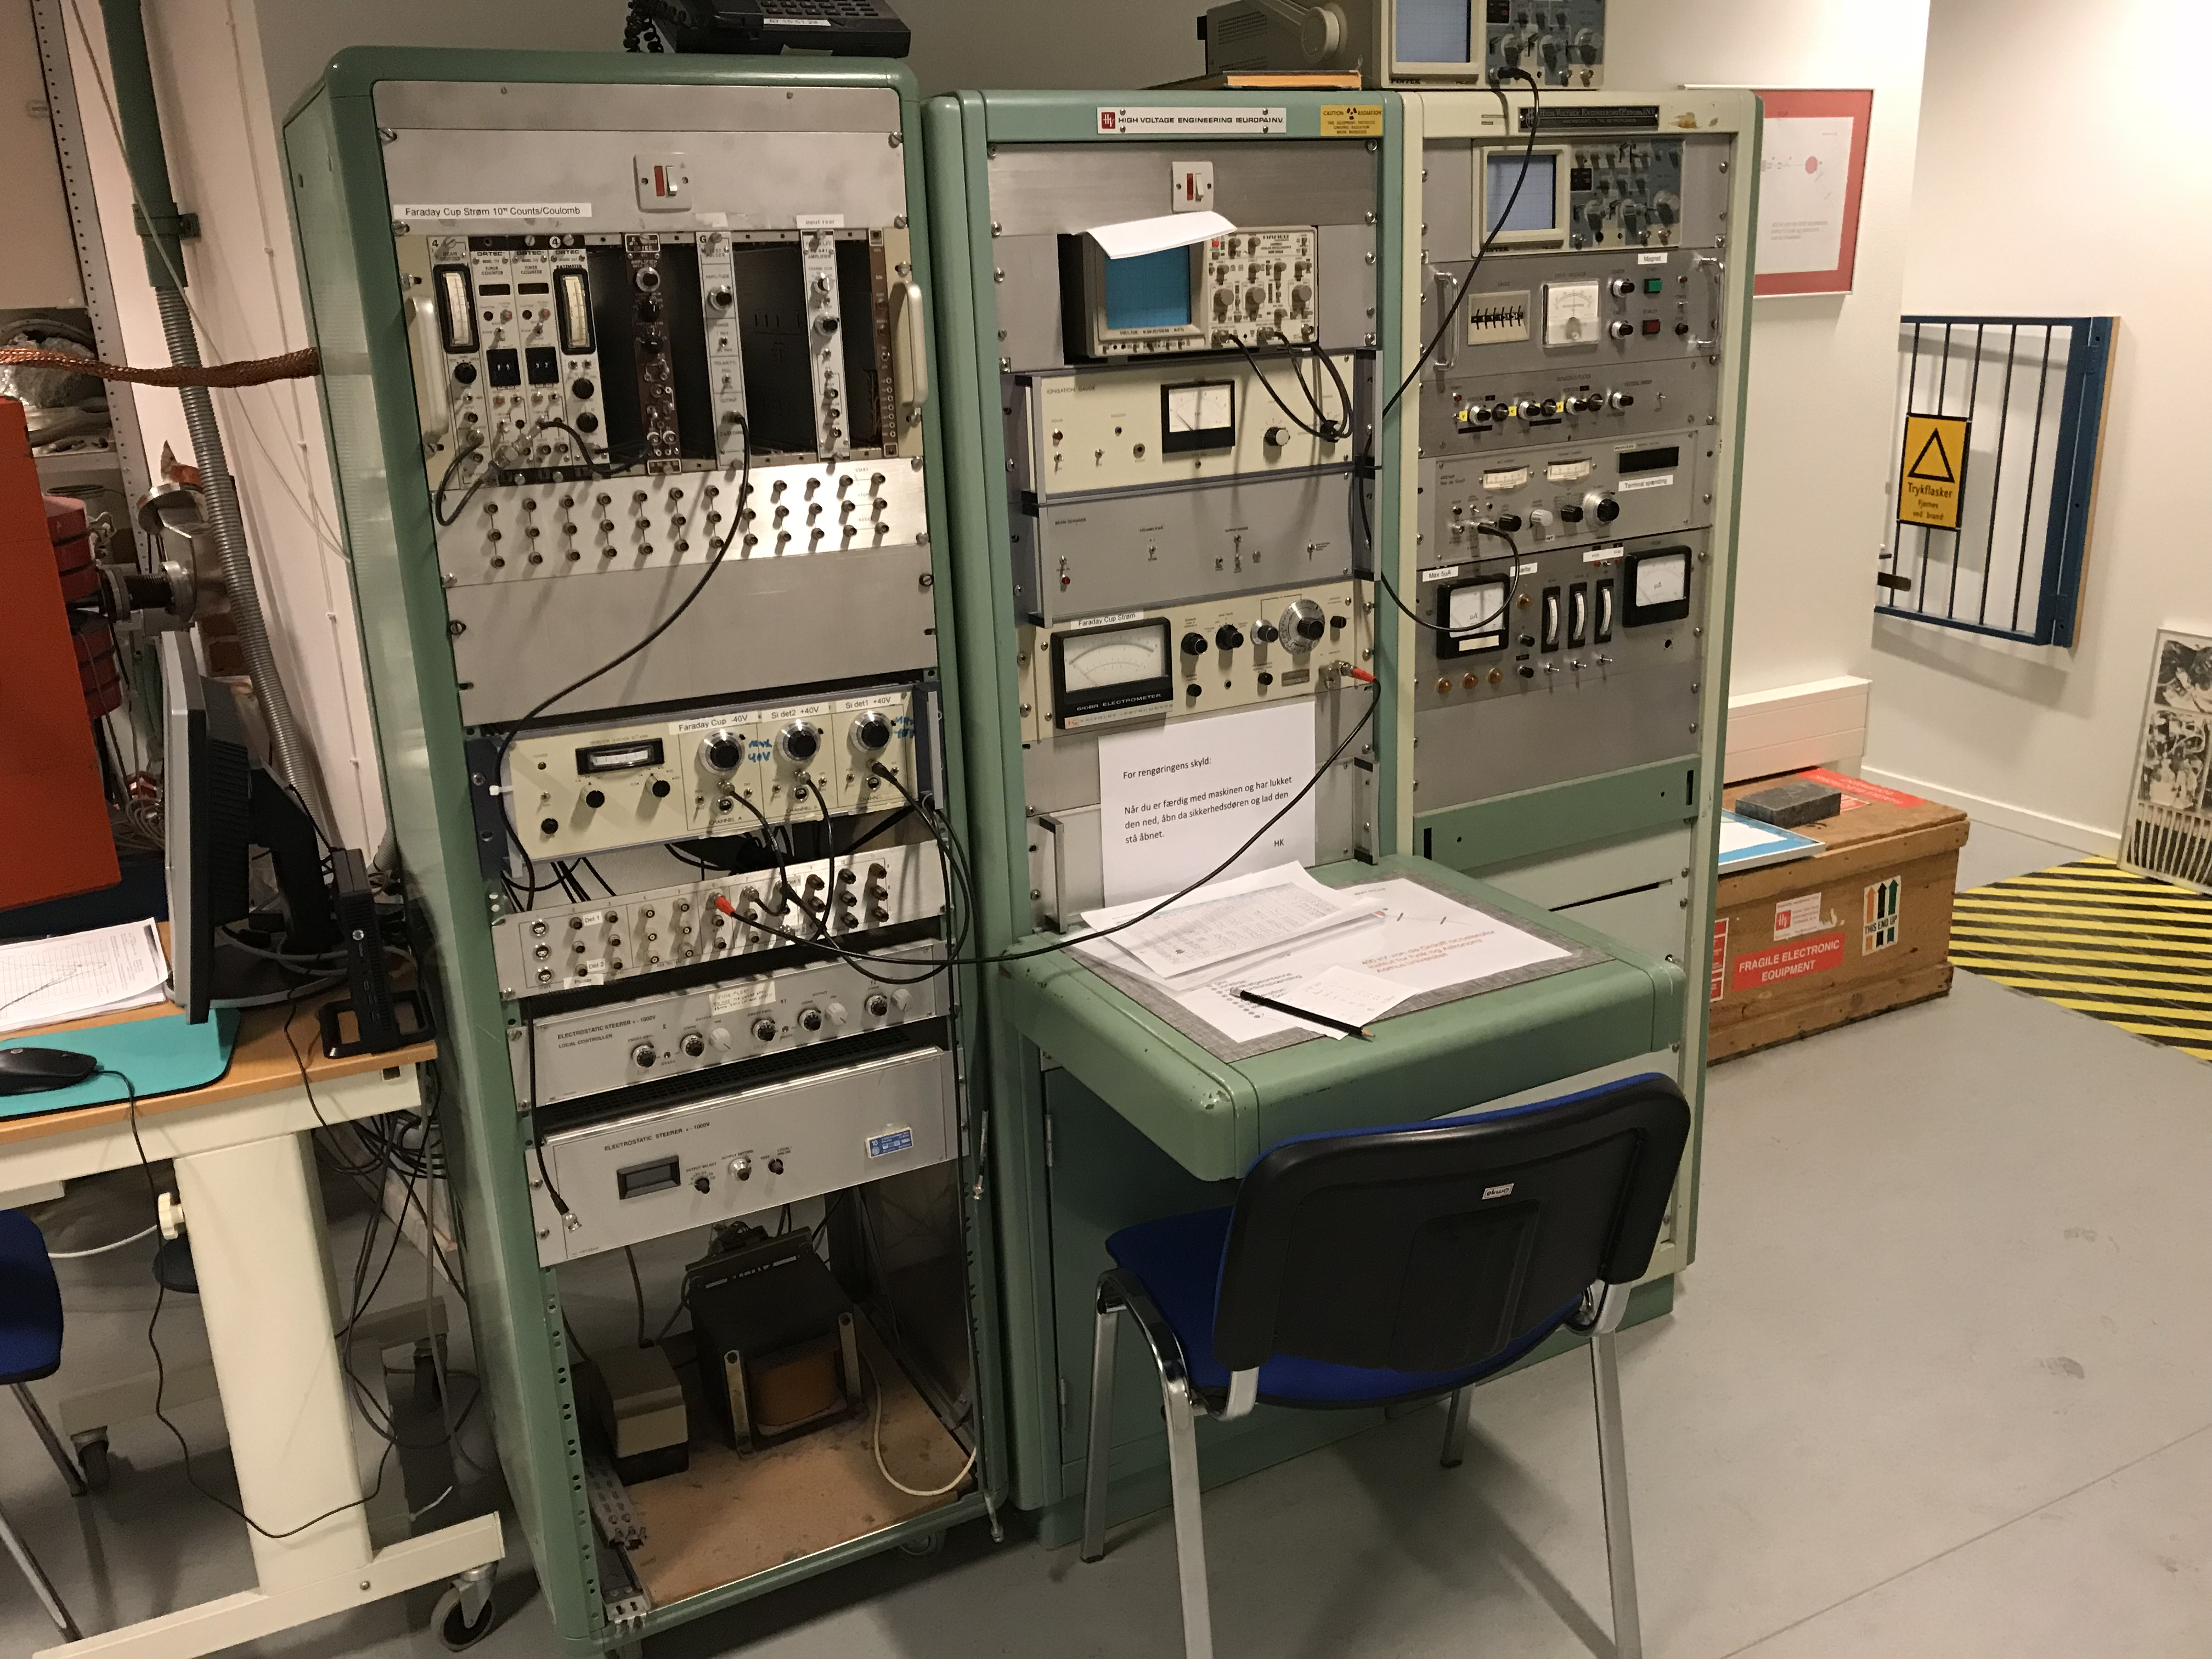
\includegraphics[width=0.99\columnwidth]{setup2}
    \caption{Overview of dashboard. Closer graphics are seen in the Procedure.}
    \label{fig_setup2}
\end{figure}
%
\begin{figure}[t]
    \centering
    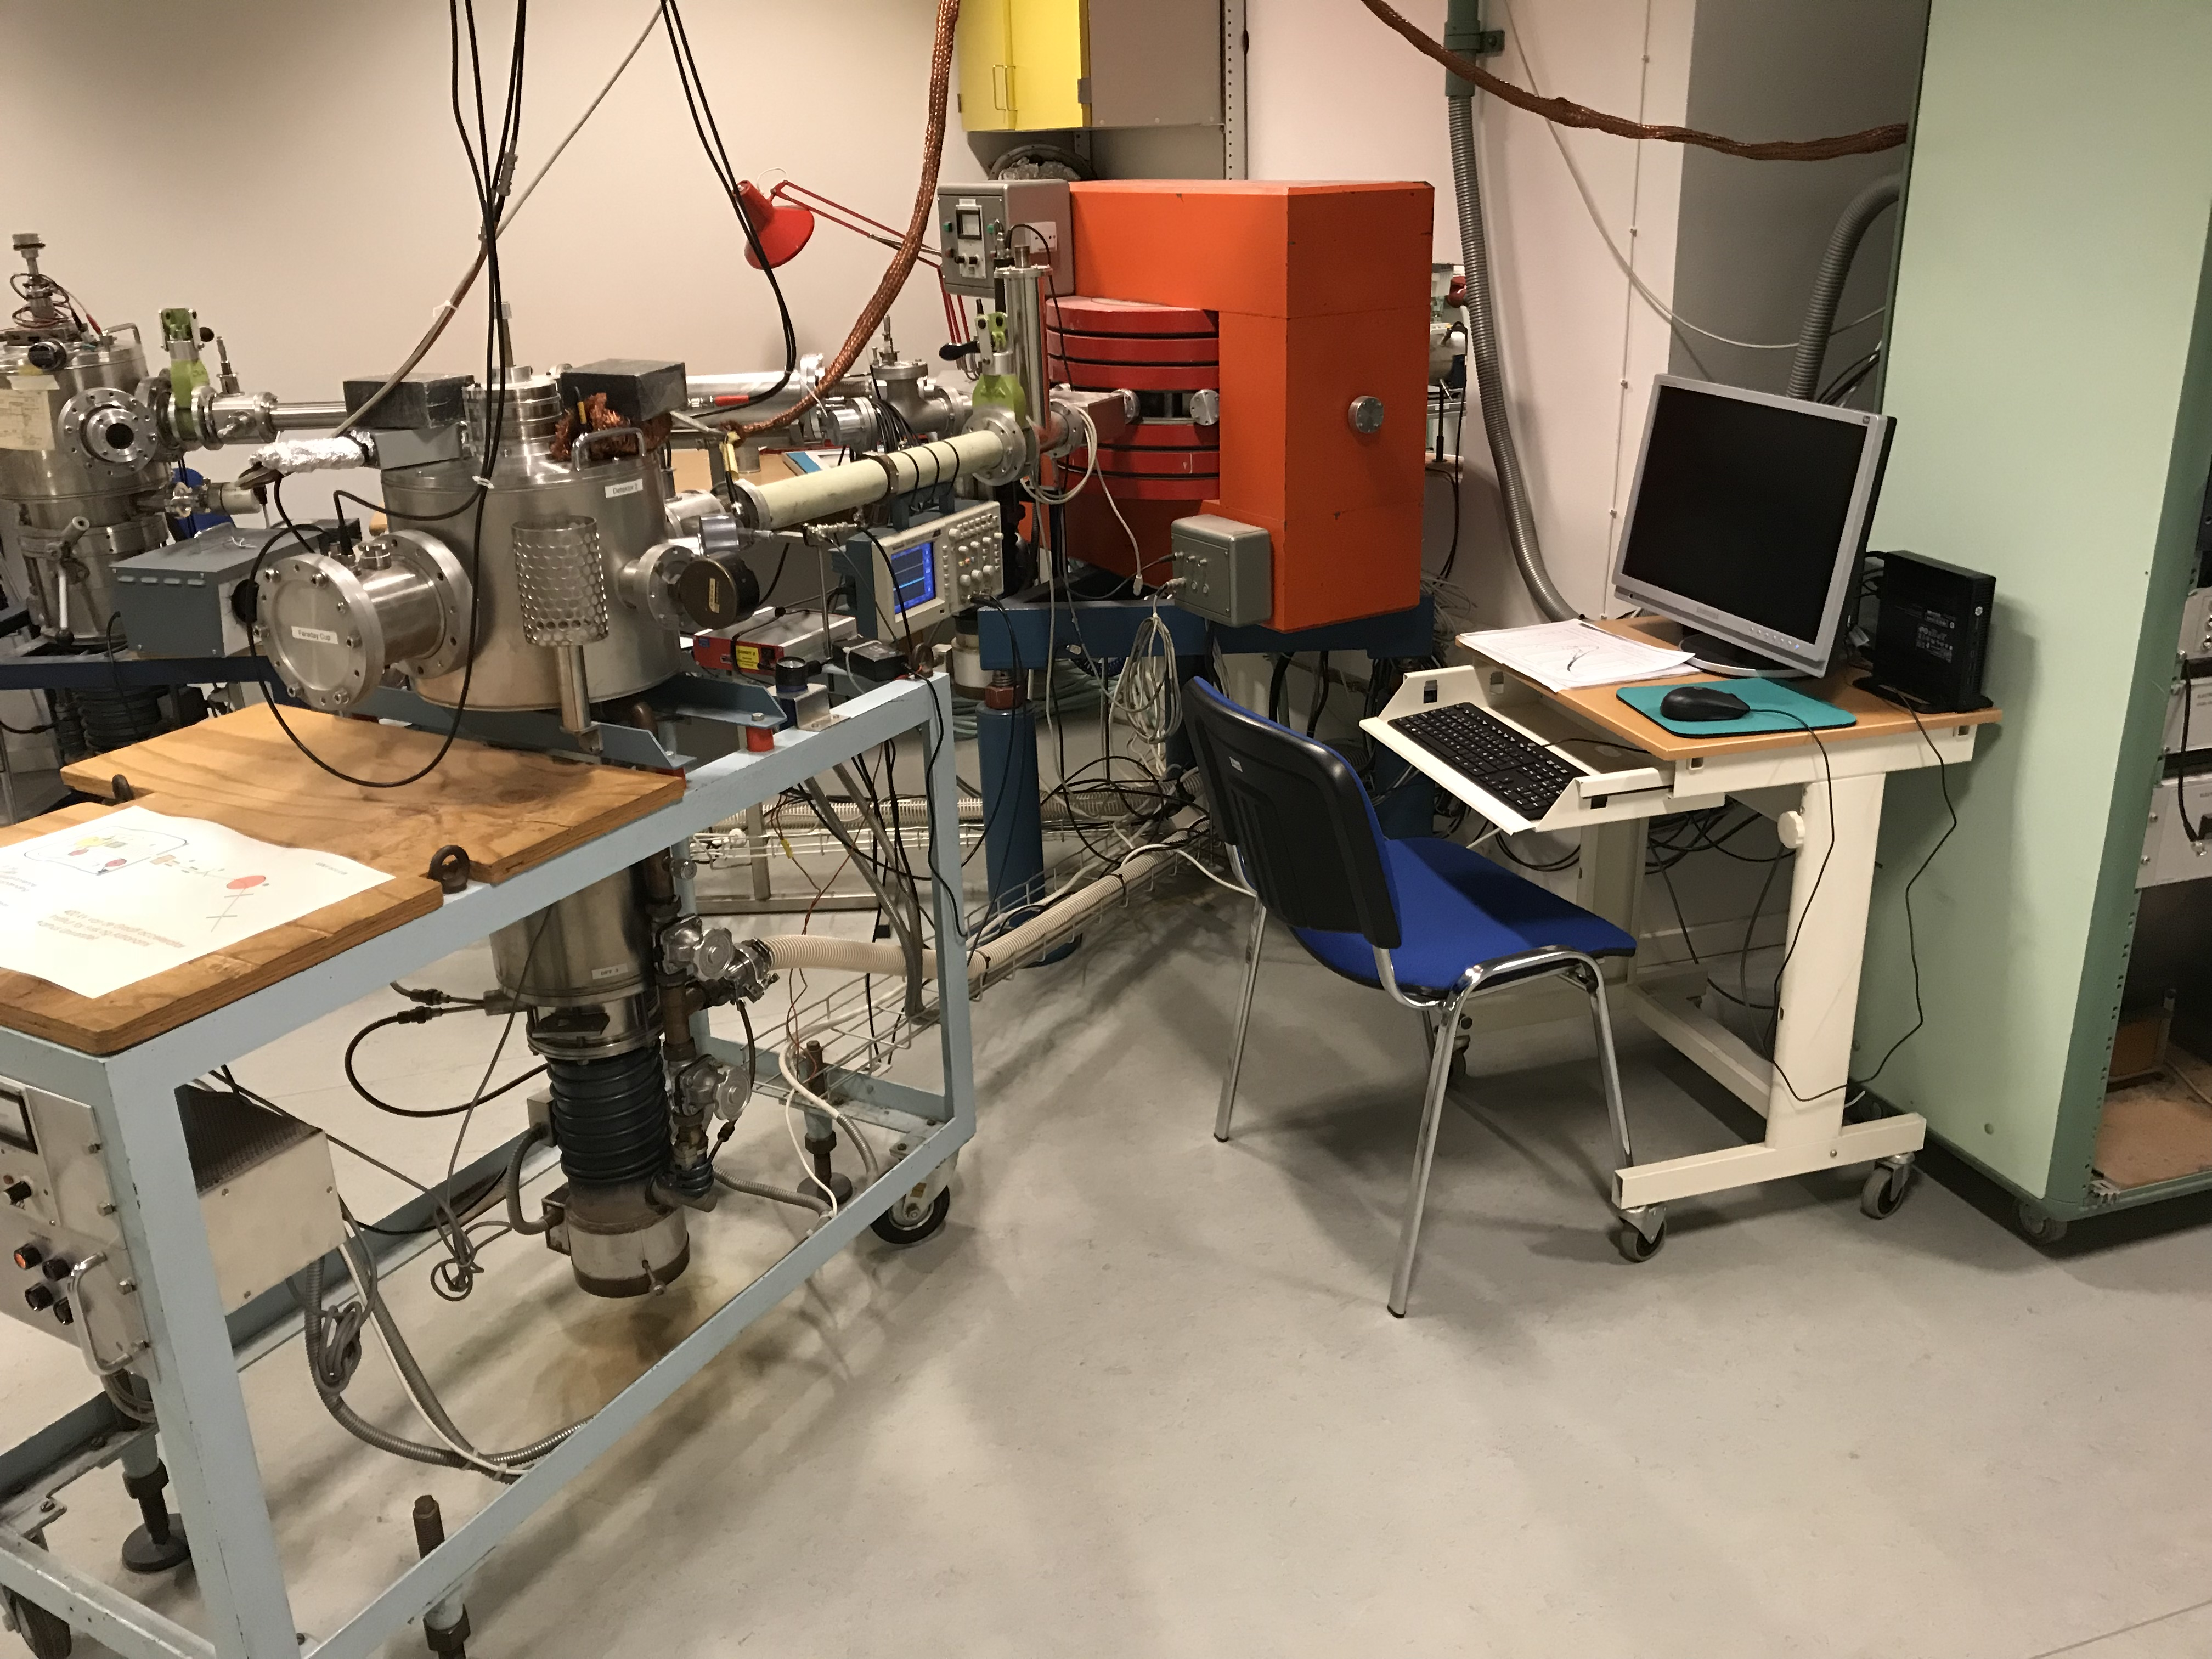
\includegraphics[width=0.99\columnwidth]{setup1}
    \caption{Overview of detector and electromagnet (red brick).}
    \label{fig_setup1}
\end{figure}
%
\begin{figure}[t]
    \centering
    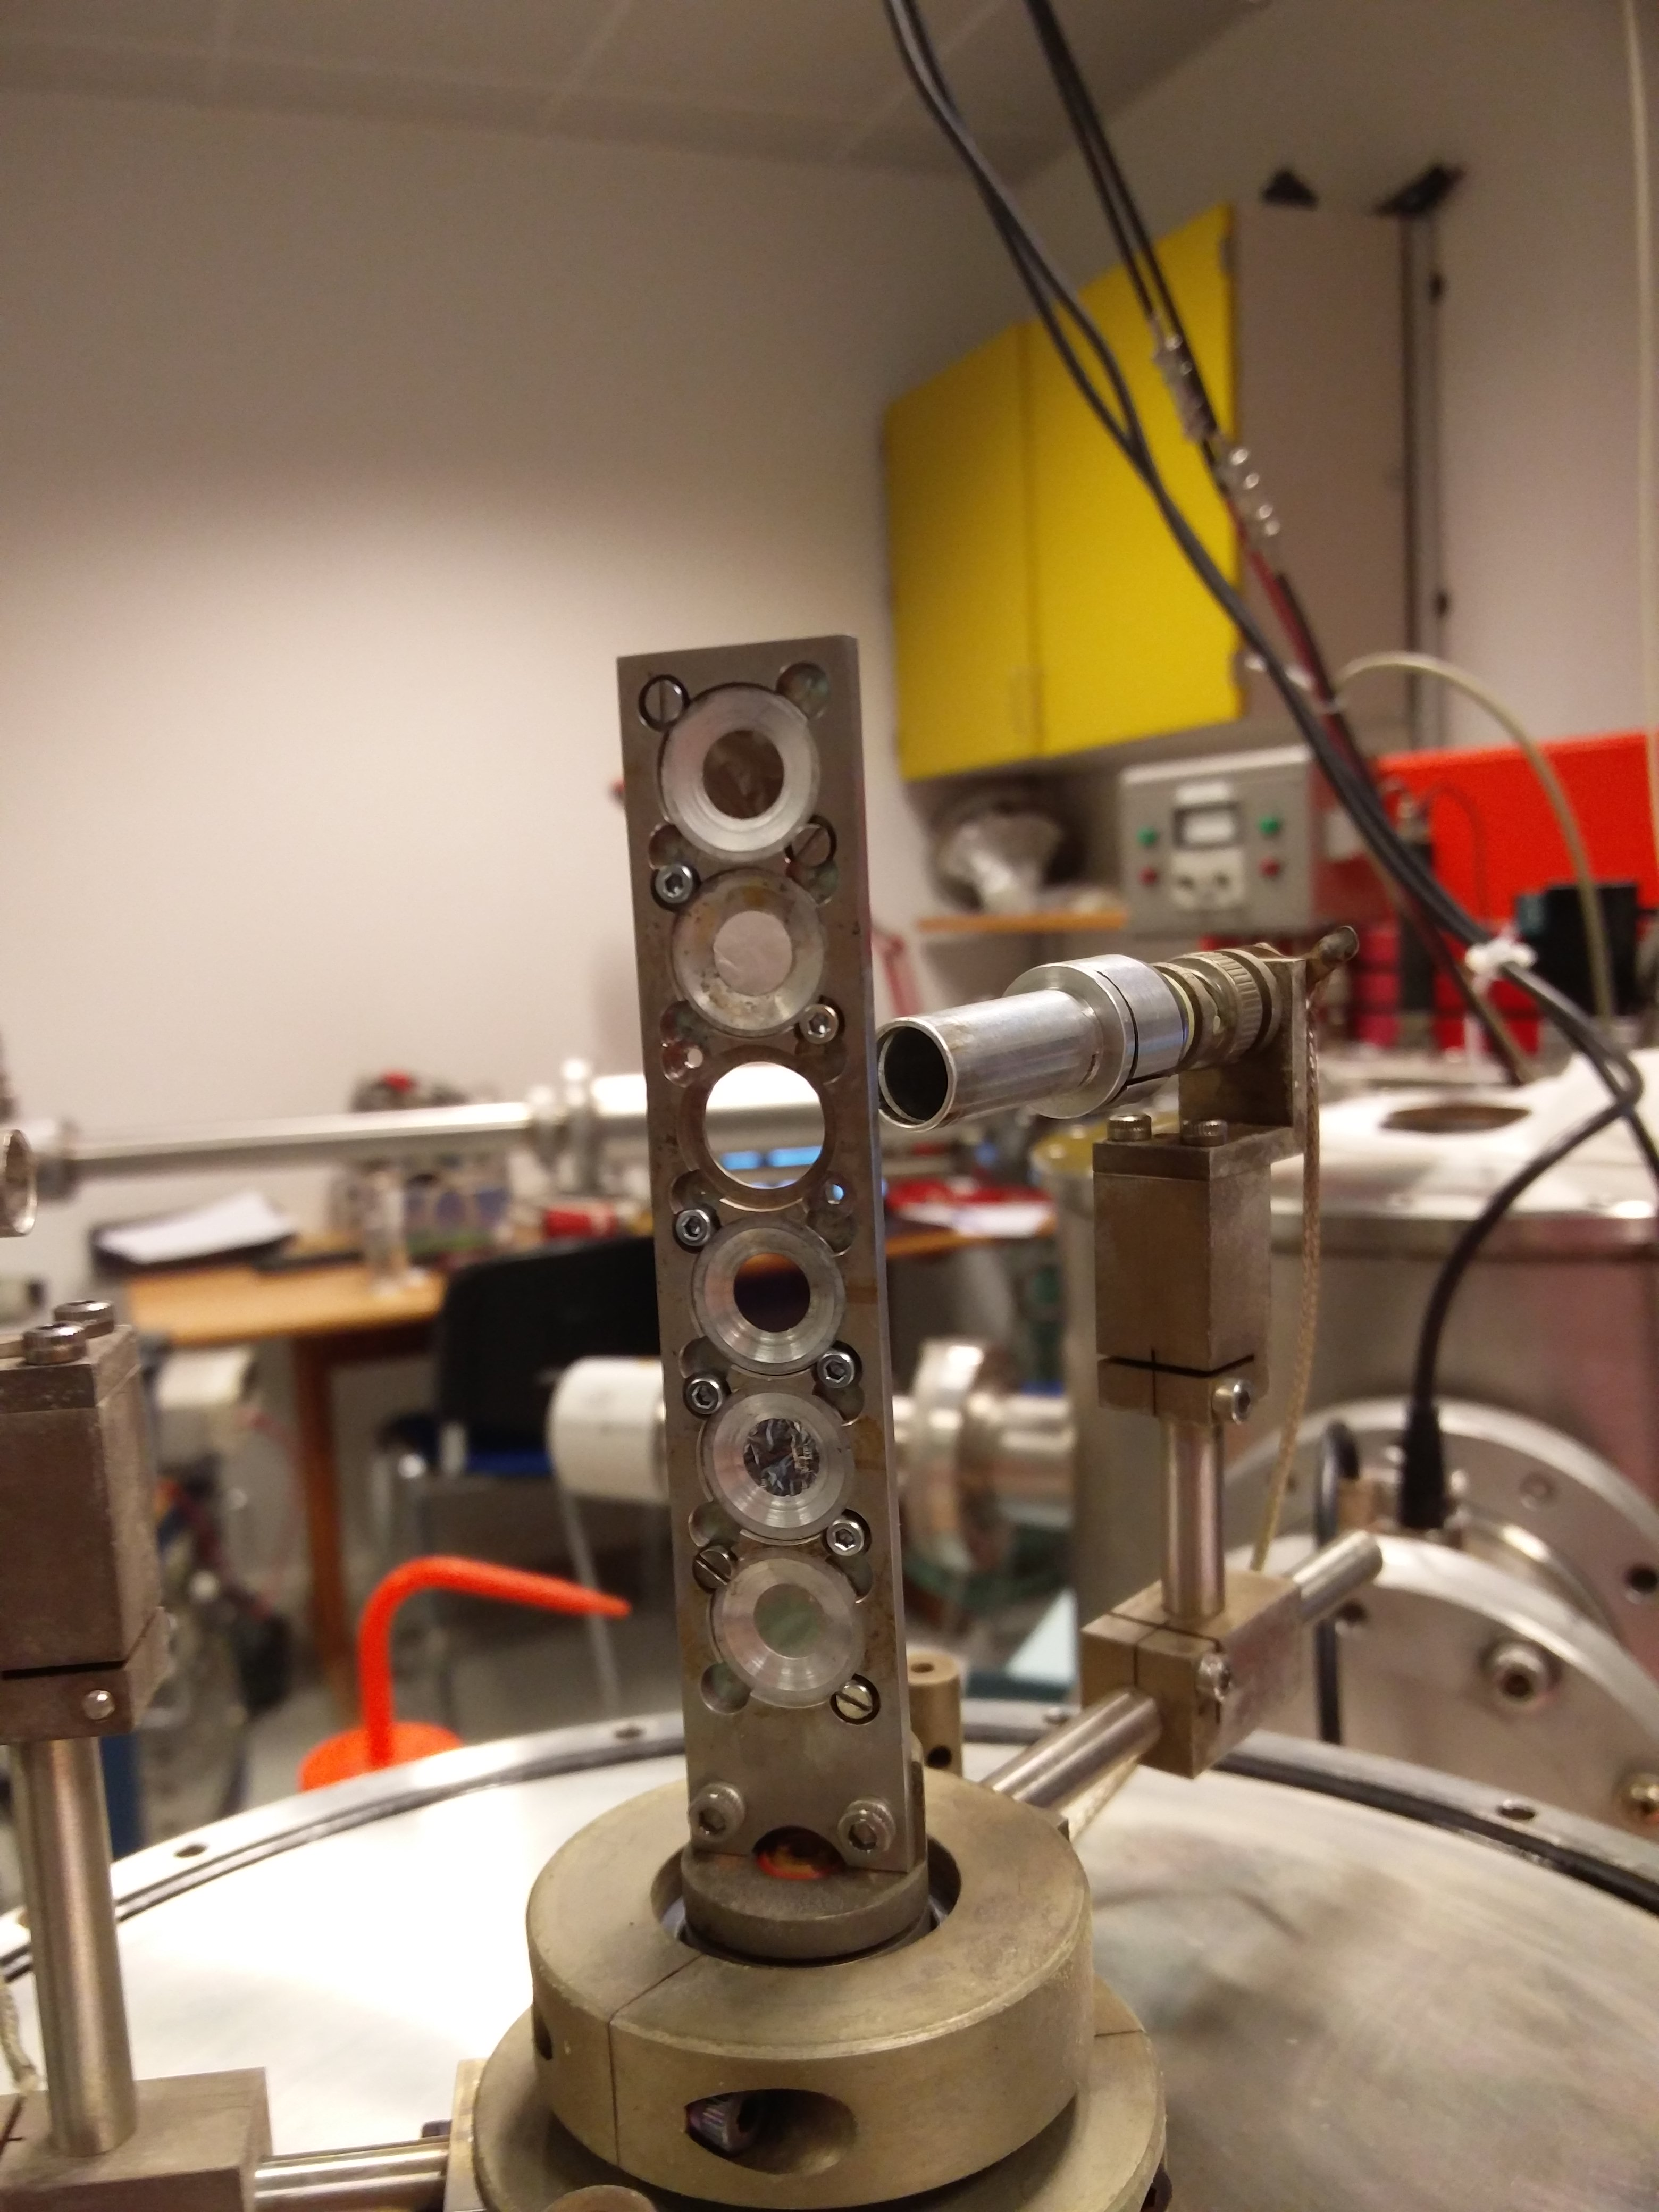
\includegraphics[trim={0cm, 10cm, 0cm, 40cm}, clip, width=0.99\columnwidth]{setup4}
    \caption{The equipment had a failure, so the targets were changed. We were
    lucky to get this picture of both detector and targets.}
    \label{fig_setup4}
\end{figure}
%
From the beamline the particles were directed toward a chosen target material
(see \cref{fig_setup4}), where they were scattered on atomic nuclei of the
target. A detector was placed at a movable position around the target, such
that scattering angles up $160$ degrees could be measured.

% % % % % % % % % % % % % % % % % % % % % % % % % % % % % % % % % % % % % % % % 
The detector was coupled to a digitizer with a time resolution of
$\SI{123}{\seconds}$\fxnote{HUSK DETTE!}  and  connected to a computer. During
measurements the digitizer started a clock inside it. When the detector was hit
by a particle, the digitizer translated the measured energy into a digital
number and sent the number and the corresponding time stamp to the computer.
The program Mc2Analyzer was used to handle the data. The digital number is an
arbitrary number called a channel number. It is translatable to the actual
energy by a linear factor plus an offset. In order to convert these channel
numbers to correct energies of the scattered particles a calibration was done.
% % % % % % % % % % % % % % % % % % % % % % % % % % % % % % % % % % % % % % % % 

\subsection{Calibration}
An energy meassurement of the scattered ion gives a digitial output, which we call
a channel number (or bin number). These hold no physical interpretation, but
can be translated to the equivalent energy of the scattered particle. To
convert these channel numbers, a calibration is necesarry. 

Assuming a linear relationship between the energy and the channel number the
energy can be found as
\begin{equation}
E = \alpha(k - k_0),
\end{equation}
where $k$ is the meassured channel and $k_0$ and $\alpha$ are parameters. The
parameters in the relation is determined by a two step program.

\subsubsection{Determing Zero-Amplitude constant}
First, by connecting a pulser (variable output voltage), a relation between the
varied energy and the corresponding channel number is obtained. 
We did this for equidistant pulsed energies, but also the lowest threshold
energy. Plotting the count numbers as a function of bin numbers, and fitting a
gaussian to each value of pulsed energy, one would obtain all parameters of the
gaussian (amplitude, mean value and standard deviation), which was used to
estimate the mean bin number, within an uncertainty of the gaussian standard deviation (see
\cref{fig_gaussian_fit}). 

Afterwards, each mean channel number was plotted as a function of the pulser
energy, and this surely shows a linear relation, which also was fitted. The
intersection is interpretated as the bin number for zero amplitude ($k_0$). A
plot can be seen on \cref{fig_linear_fit}.

%\cref{fig_gaussian_fit}  shows the count distribution as function of channels for the amplitude fitted with gaussian function. The data clearly follows a gaussian distribution and the data points are, within uncertainty, well described by a gausian distribution. 

%However, another method is used to determine the zero-amplitude constant $k_0$. Different energies are generated using a pulse generator by changing the amplitude (corresponding to a change of resistance). For each fixed amplitude, a normal distribution of counts around a certain mean channel is obtained. The mean channel (also called the centroid) is determined from a Gaussian fit to the distribution. 

\begin{figure}[h]
\centering
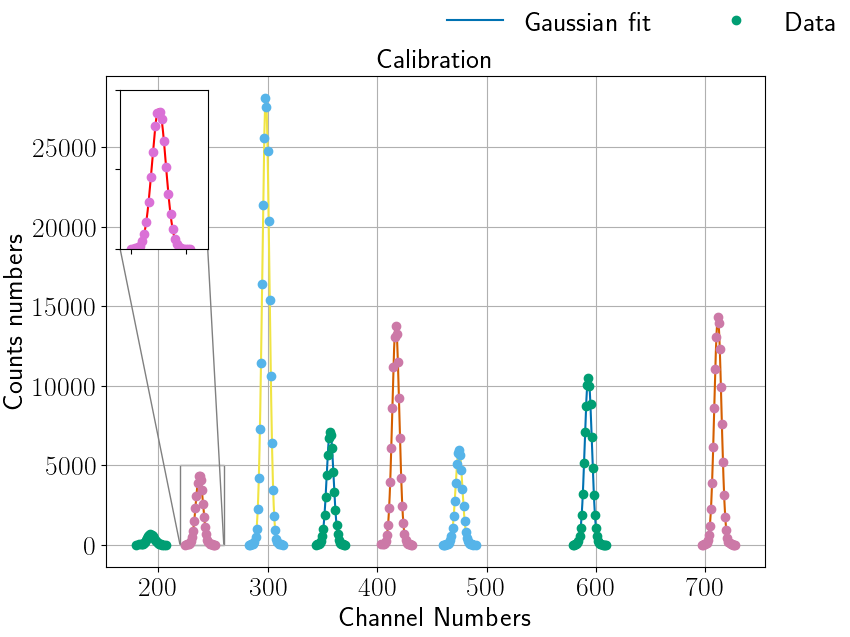
\includegraphics[width=0.99\columnwidth]{gaussian_fit}
\caption{Gaussian fit of all data values. This was used to estimate the mean
bin number (channel number), and the uncertainty of this bin number, in the
energy-calibration.}
\label{fig_gaussian_fit}
\end{figure}

\begin{figure}[h]
\centering
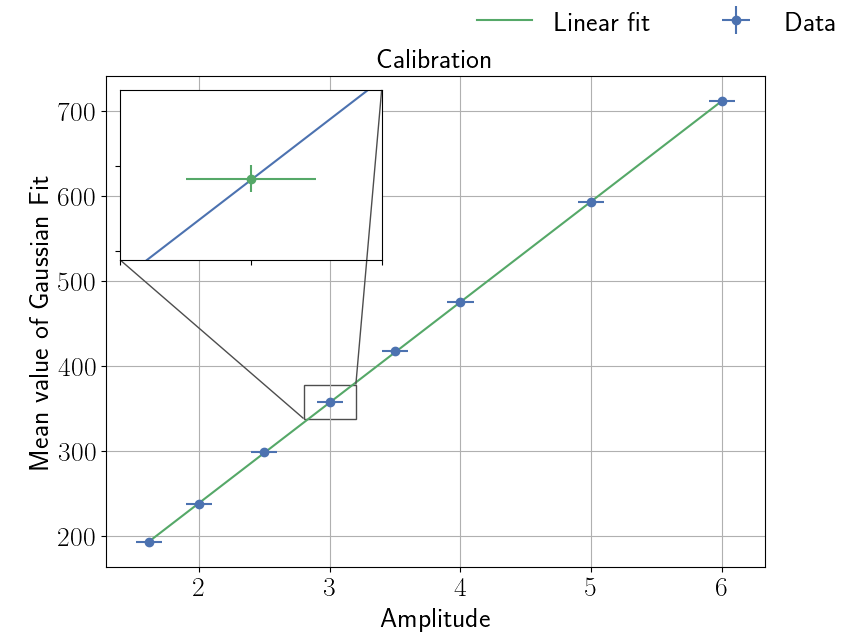
\includegraphics[width=0.99\columnwidth]{k0_plotting}
\caption{Linear fit of the mean values as a function of amplitude. This was
used to determine the zero-amplitude constant $k_0$.}
\label{fig_linear_fit}
\end{figure}

\subsubsection{Determining alpha}
As described in the previous section, the magnetic field strength of the
electromagnet can be adjusted to deflect either $\mathrm{H^+}$ or
$\mathrm{{H_2}^+}$ into the beamline. For each of these a data point of energy
related to channel number can be found.
By considering energy and momentum conservation for elastic scattering in two
dimensions the energy of the scattered particles $E_f$ can be found from the
incident proton energy and the scattering angle as:
\begin{equation}
E_f = \left( \frac{m_|p| \cos\theta + \sqrt{{m_|t|}^2 - {m_|p|}^2
\sin^2\theta}}{m_|p|+m_|t|} \right)^2 E_|i|,
\end{equation}
where $E_|i|$ is the energy of the incident beam particles, $m_|p|$ and $m_|t|$ are
the masses of the incident protons and the target particles, respectively, and
$\theta$ is the angle between the direct outgoing non-scattered beam and the
scattered particles - also called the scattering angle.

Unfortunately, this only give two data points one from $\mathrm{H^+}$ and
another from $\mathrm{{H_2}^+}$. Nonetheless, the incline from the linear fit
to these data points is still useful.

\begin{figure}[t]
\centering
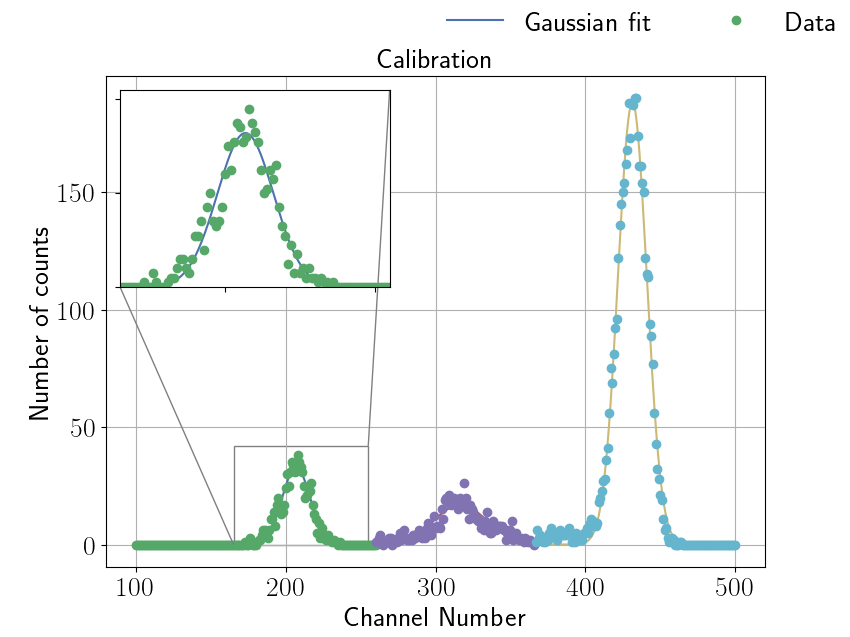
\includegraphics[width=0.99\columnwidth]{gaussian_fit2}
\caption{Gaussian fit of all data values. This was used to estimate the mean
bin number (channel number), and the uncertainty of this bin number, in the
energy-calibration.}
\label{fig_gaussian_fit2}
\end{figure}

\begin{figure}[t]
\centering
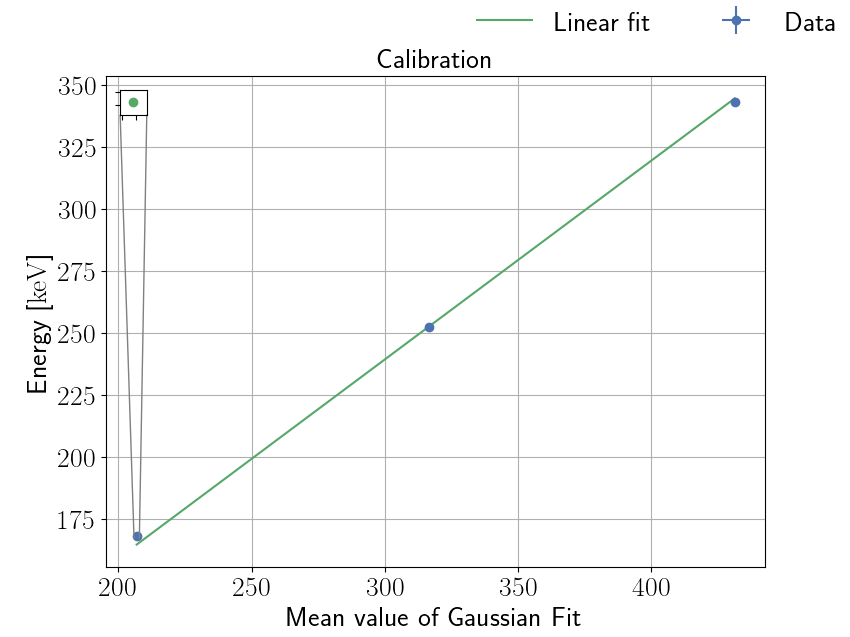
\includegraphics[width=0.99\columnwidth]{alpha_plotting}
\caption{Linear fit of the mean values as a function of amplitude. This was
used to determine the zero-amplitude constant $k_0$.}
\label{fig_linear_fit2}
\end{figure}




%TABLE WITH CORRESPONDING VALUES OF AMPLITUDE AND MEAN CHANNEL (AND THEIR UNCERTAINTIES)!
%
%FIGURE WITH AN EXAMPLE OF A GAUSSIAN FIT.

%From the fit the coefficient $k_0$ is .... 
%
%
%
%\subsection{Targets}
%Something about the different targets... Rettes til når vi ved noget mere.
%
%The targets and their corresponding thickness and areal density are noted in Table ...
%
%%\begin{table}[h]
%%\centering
%%\caption{\sl De maalte data for kalibreringen af....}
%%\begin{tabular}{l D{.}{,}{5.0} *{2}{ D{.}{,}{10.0} @{$\pm$} D{.}{,}{2.0} } %D{.}{,}{3.0}}
%%\toprule
%% \multicolumn{1}{c}{Target} & \multicolumn{2}{c}{Thickness (Å)} & %\multicolumn{2}{c}{Area density} \\
%%\midrule
%%LiF/C  &  ?  &  ? & 0.5 \\
%%B/C  &  ?  &  ?  \\
%%AL  &  ?  &  ?  \\
%%Au/C  &  ?  &  ?  \\
%%\bottomrule
%%\end{tabular}
%%\label{tbl:eksempel}
%%\end{table}

%\subsection{Scattering on atomic nuclei}
%The aim of this experiment was to use a particle accelerator to test certain dependencies of Rutherford scattering. Numerically, the Rutherford scattering differential cross section per target atom for any target atom is
%\begin{equation}
%\frac{d\sigma}{d\Omega} = 1.296 \left( \frac{Z_1 Z_2}{E_\infty [MeV] \, \sin^2 \left(\frac{\theta}{2} \right) }\right)^2\left[\frac{mb}{sr}\right],
%\end{equation}
%where $\theta$ is the scattering angle, $Z_1$  is the atomic number of the incident particles, $Z_2$ is the atomic number of the target nuclei, and $E_{\infty}$ is their kinetic energy HUSK CITE!%cite 
%. 
%In order to test these dependencies a relation between the cross section and the count rate (number of scattered particles per time) is found as
%\begin{equation}
%dN = N \, n_{\text{tar}} \, dx \,d\Omega \, \frac{d\sigma(\theta,\phi)}{d\Omega},
%\end{equation}
%where $N$ is the number of incoming particles per time, $n_\text{tar}$ is the particle density of the target, $dx$ is the thickness of the target, and $d\Omega$ is the solid angle of the detector.
%

\clearpage
\subsection{Procedure}
First thing, the Van-de-Graaf. To accelerate the beam of incomming particles,
one has to generate a hugh potential. Turning on the Belt, one hears the
mechanical rhumming. This will generate a potential difference as described
further in \cite[p.xx]{krane}.
\begin{figure}[h]
\centering
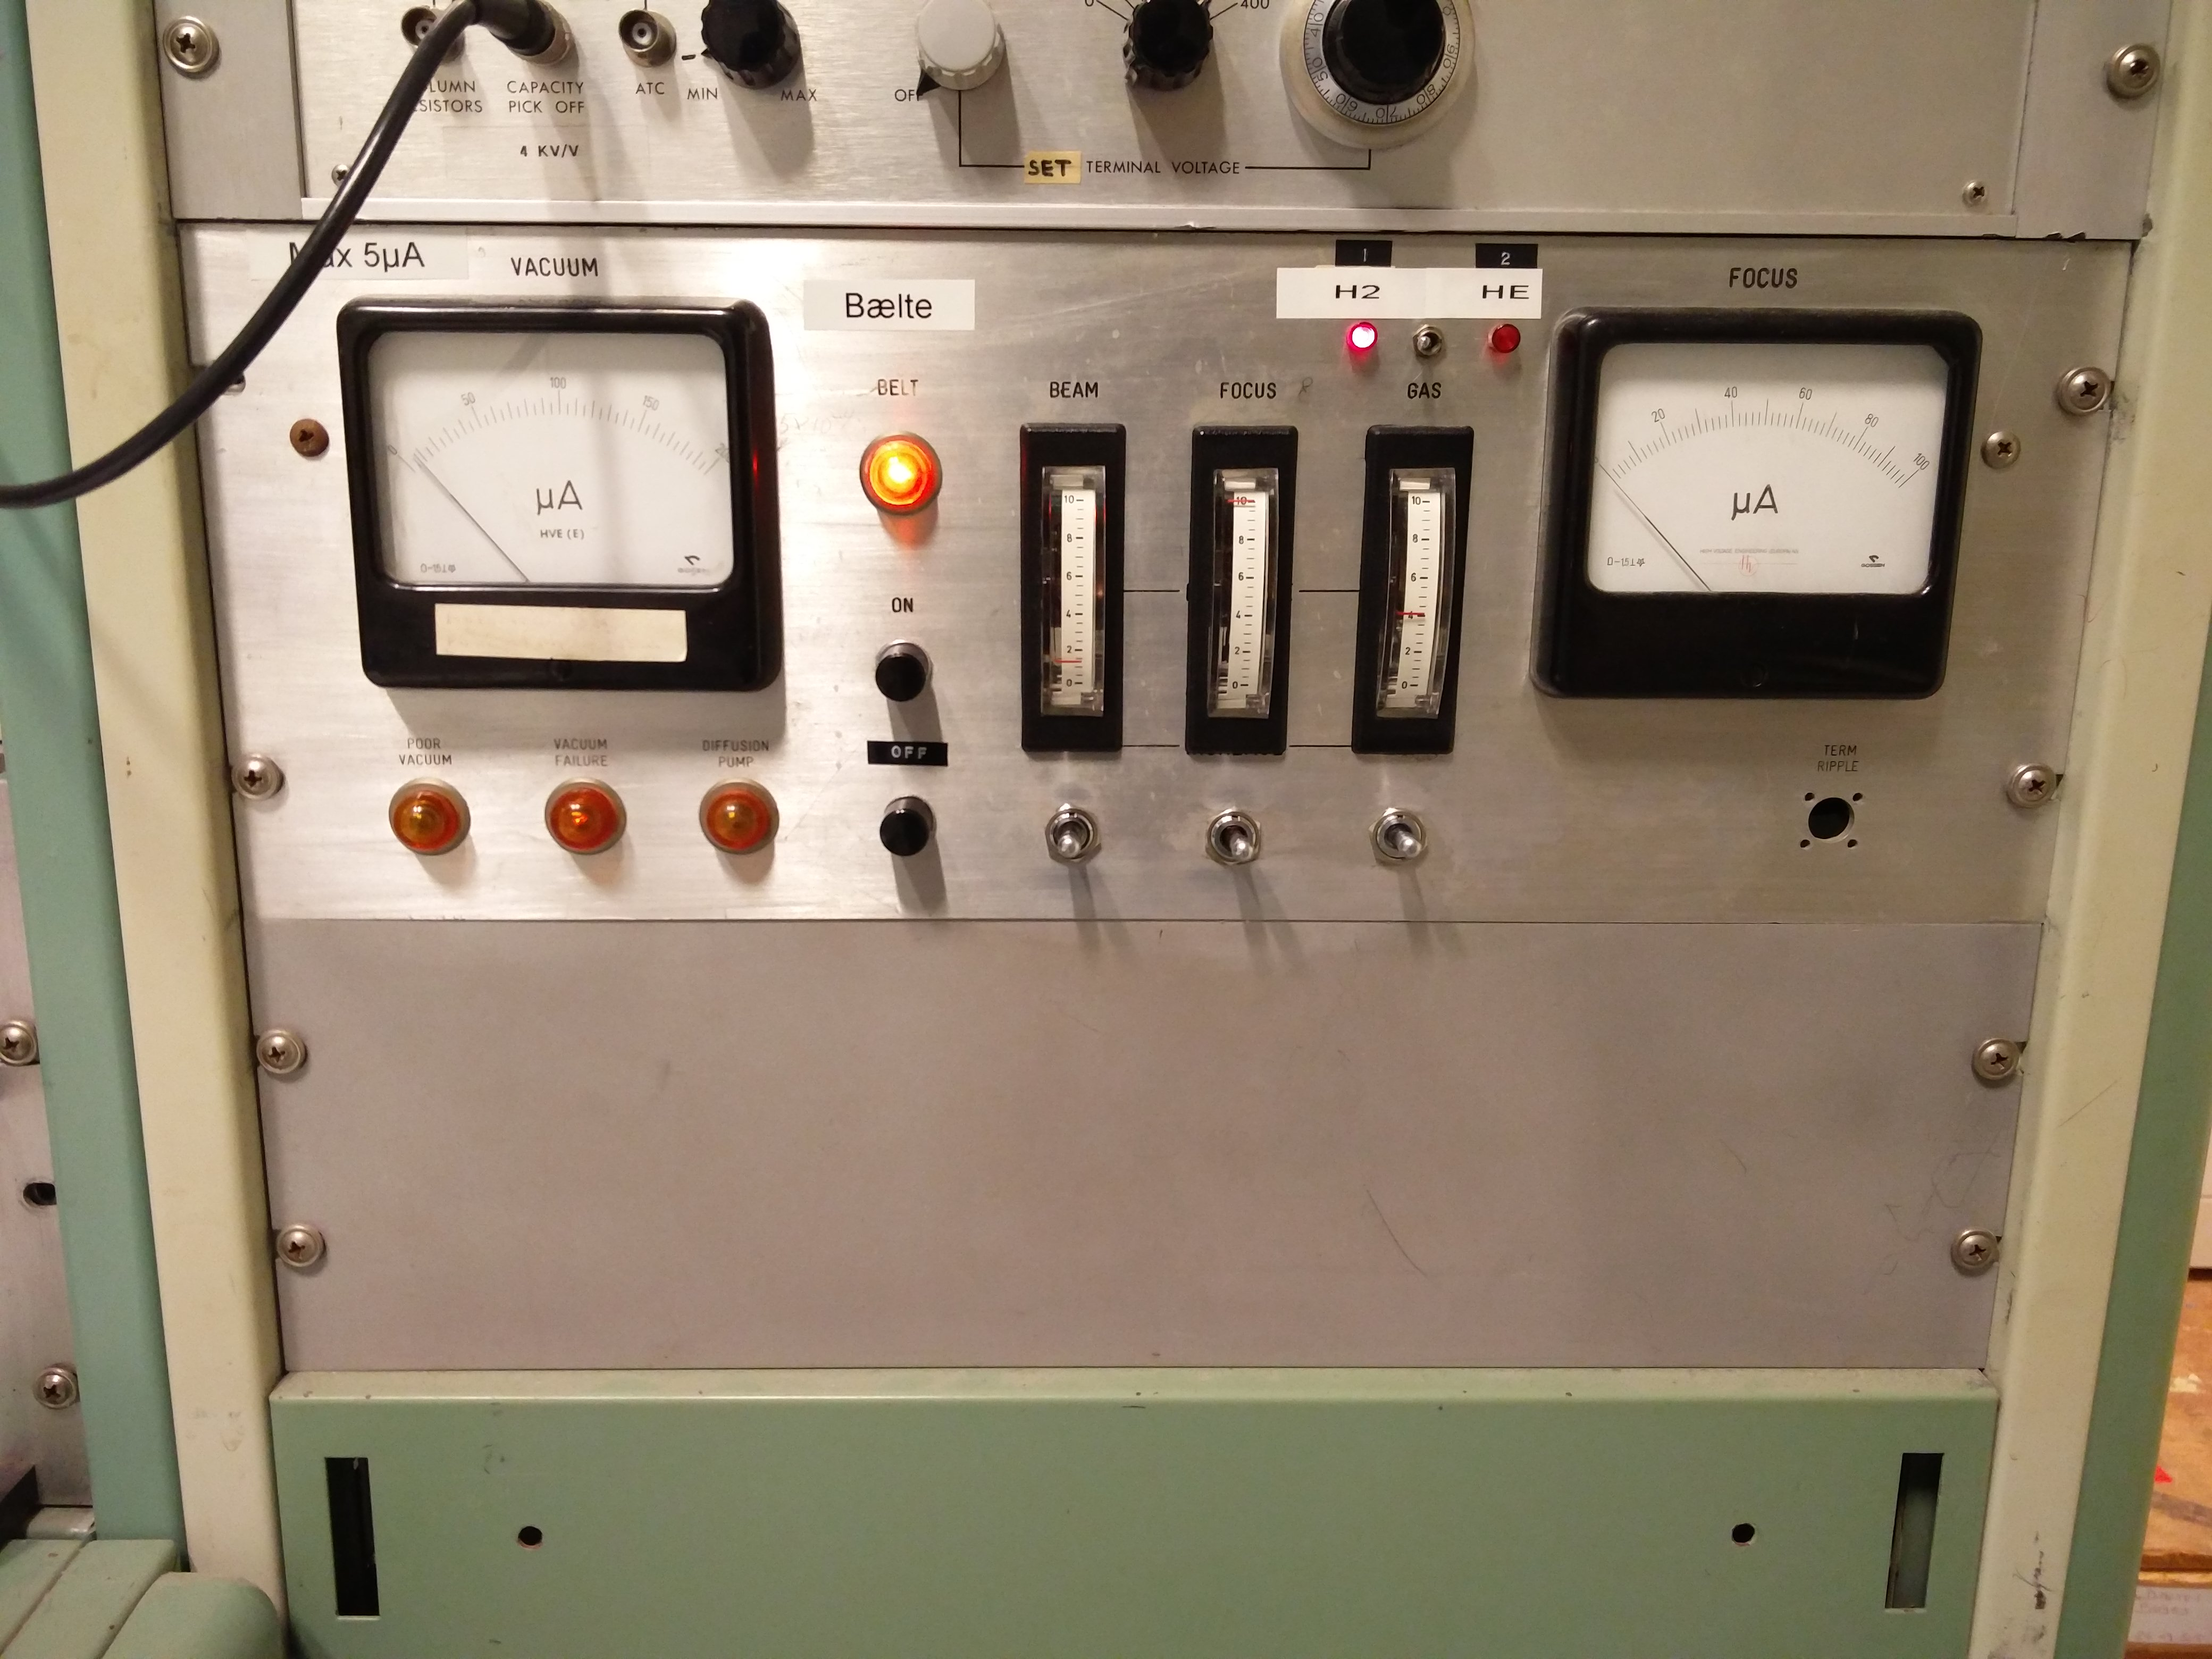
\includegraphics[trim={0, 45cm, 0, 15cm}, clip, width=0.99\columnwidth]{process1}
\caption{The belt}
\label{fig_process1}
\end{figure}

Now adjust the terminal voltage patiently towards to wanted energy. Our lab
instructor advised us to wait for each step, before going to the next.
\begin{figure}[h]
\centering
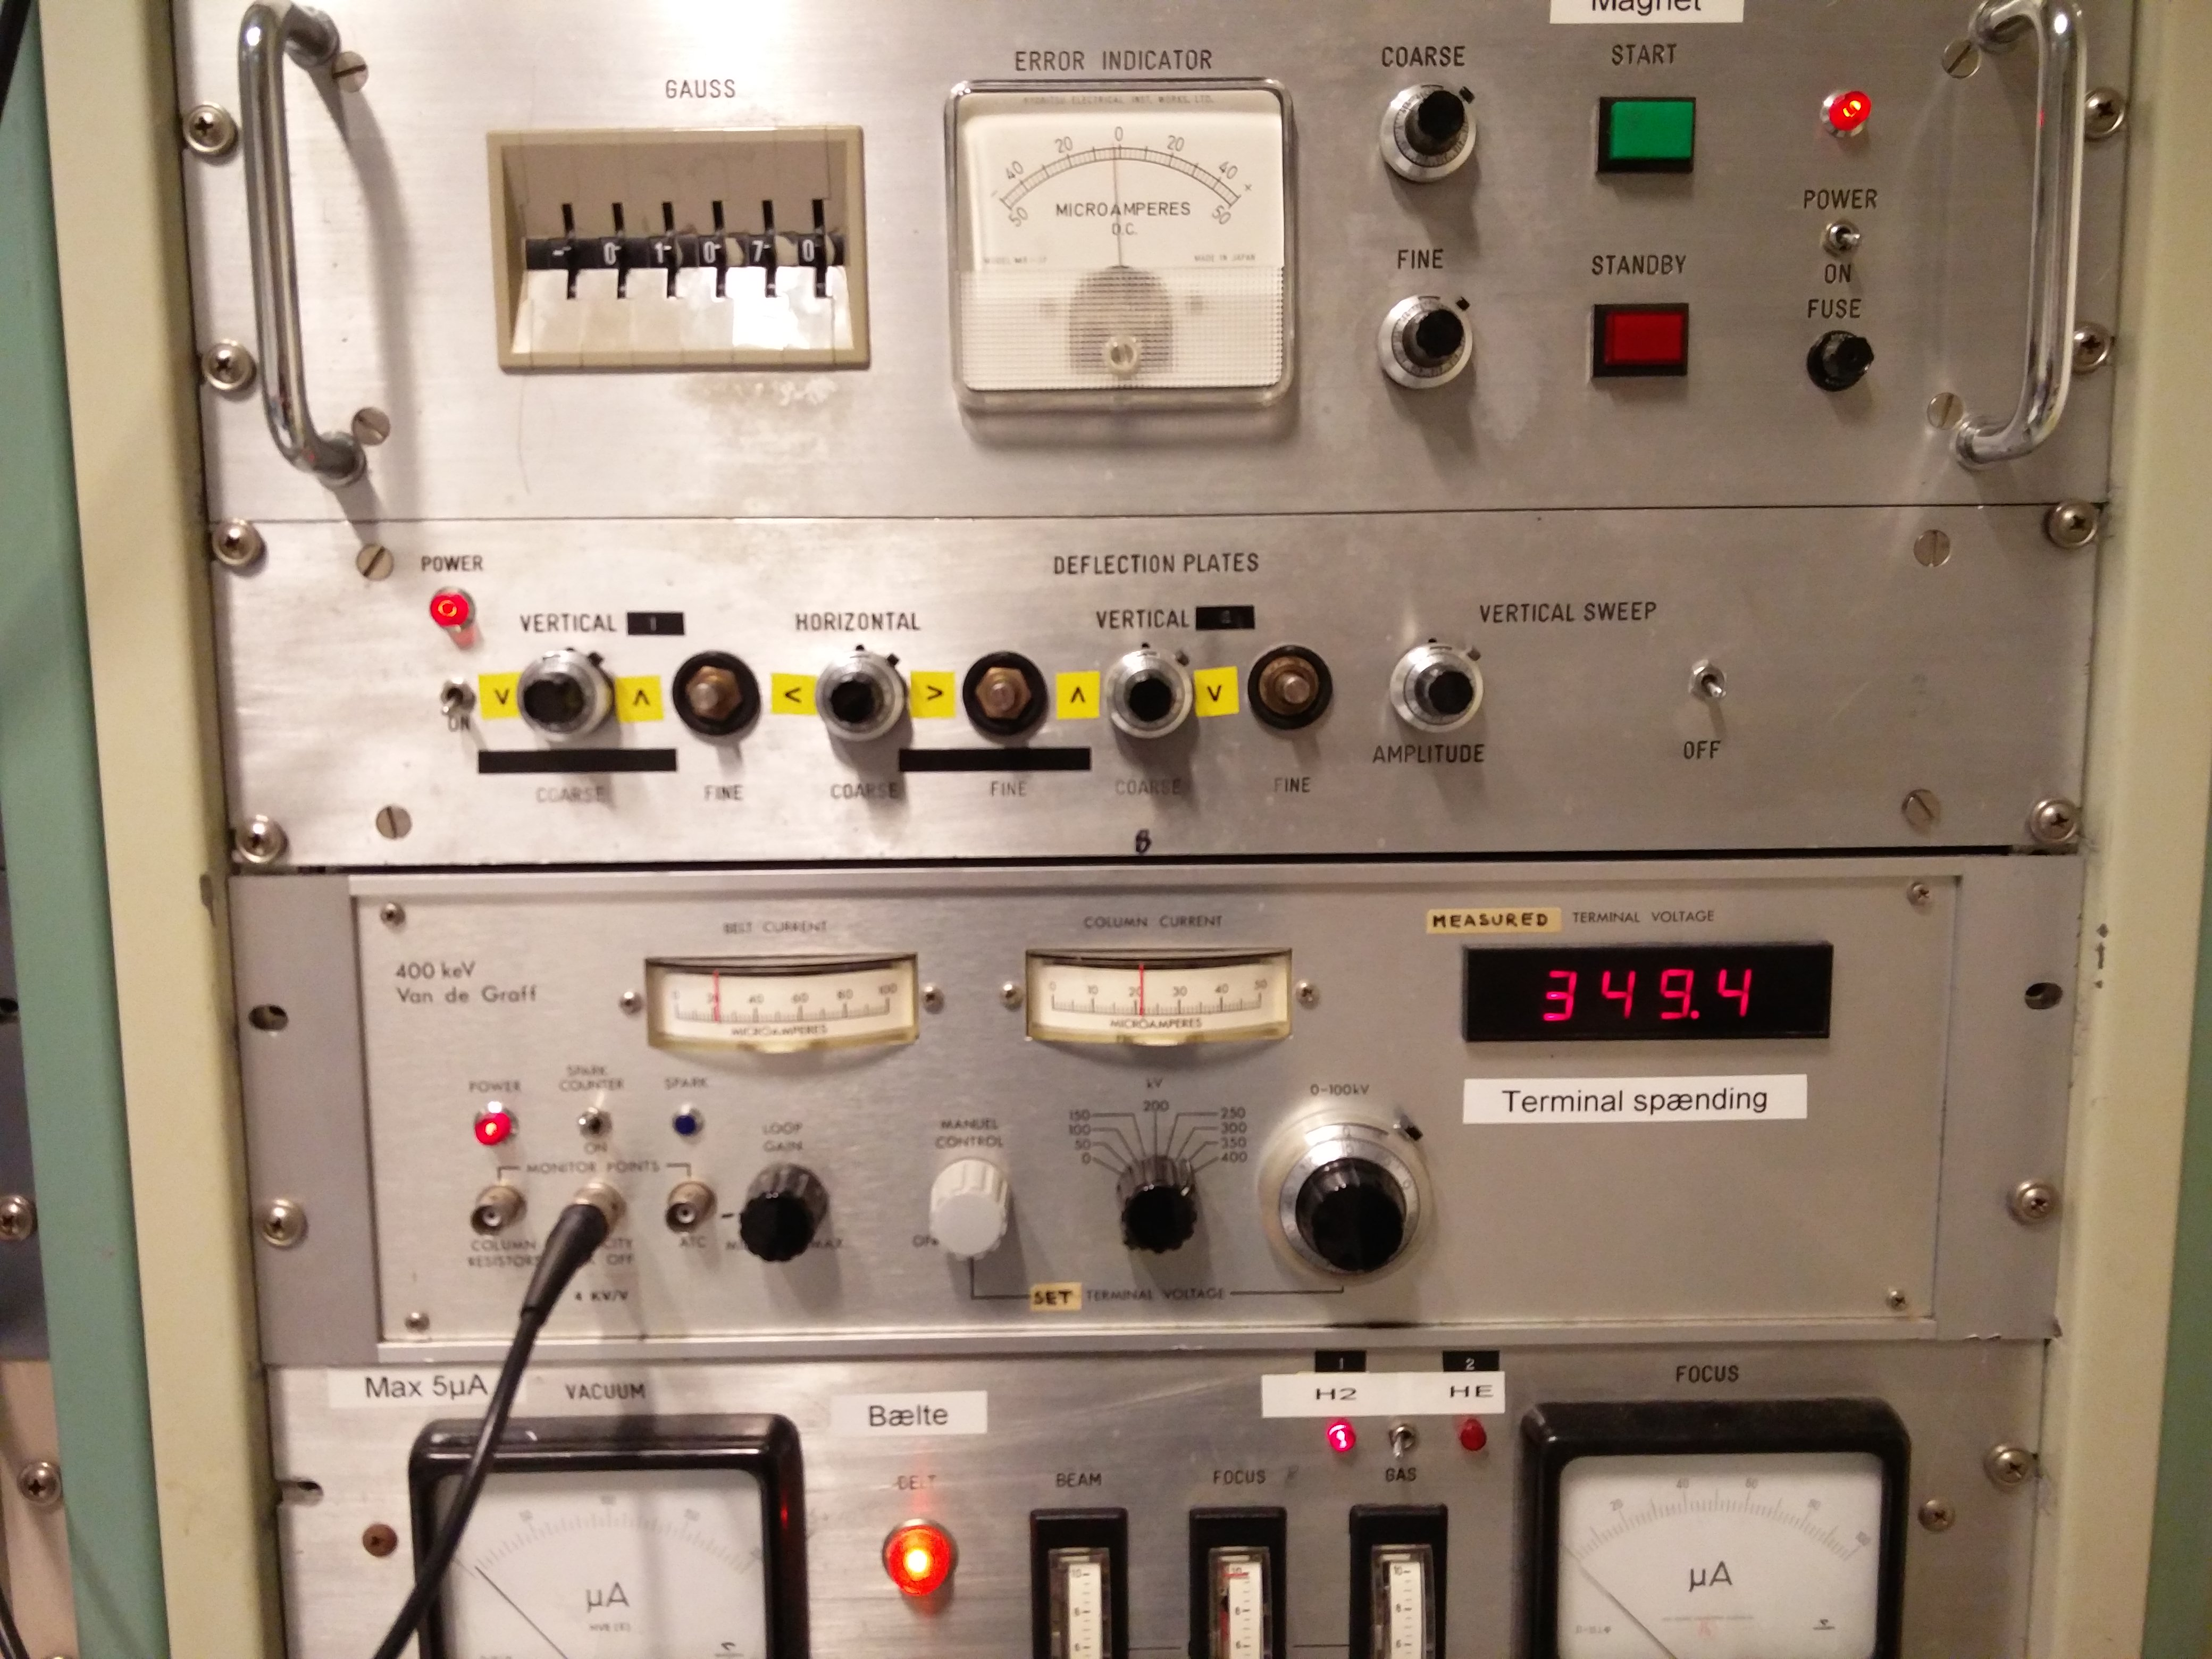
\includegraphics[trim={0, 20cm, 0, 55cm}, clip, width=0.99\columnwidth]{process2}
\caption{terminal voltage}
\label{fig_process2}
\end{figure}

Turn on the electromagnet. Remember to calculate the wanted B-field for given
element. Look on Faraday cup for received current of particles. Maximize with
fine grid (small adjustments).
\begin{figure}[h]
\centering
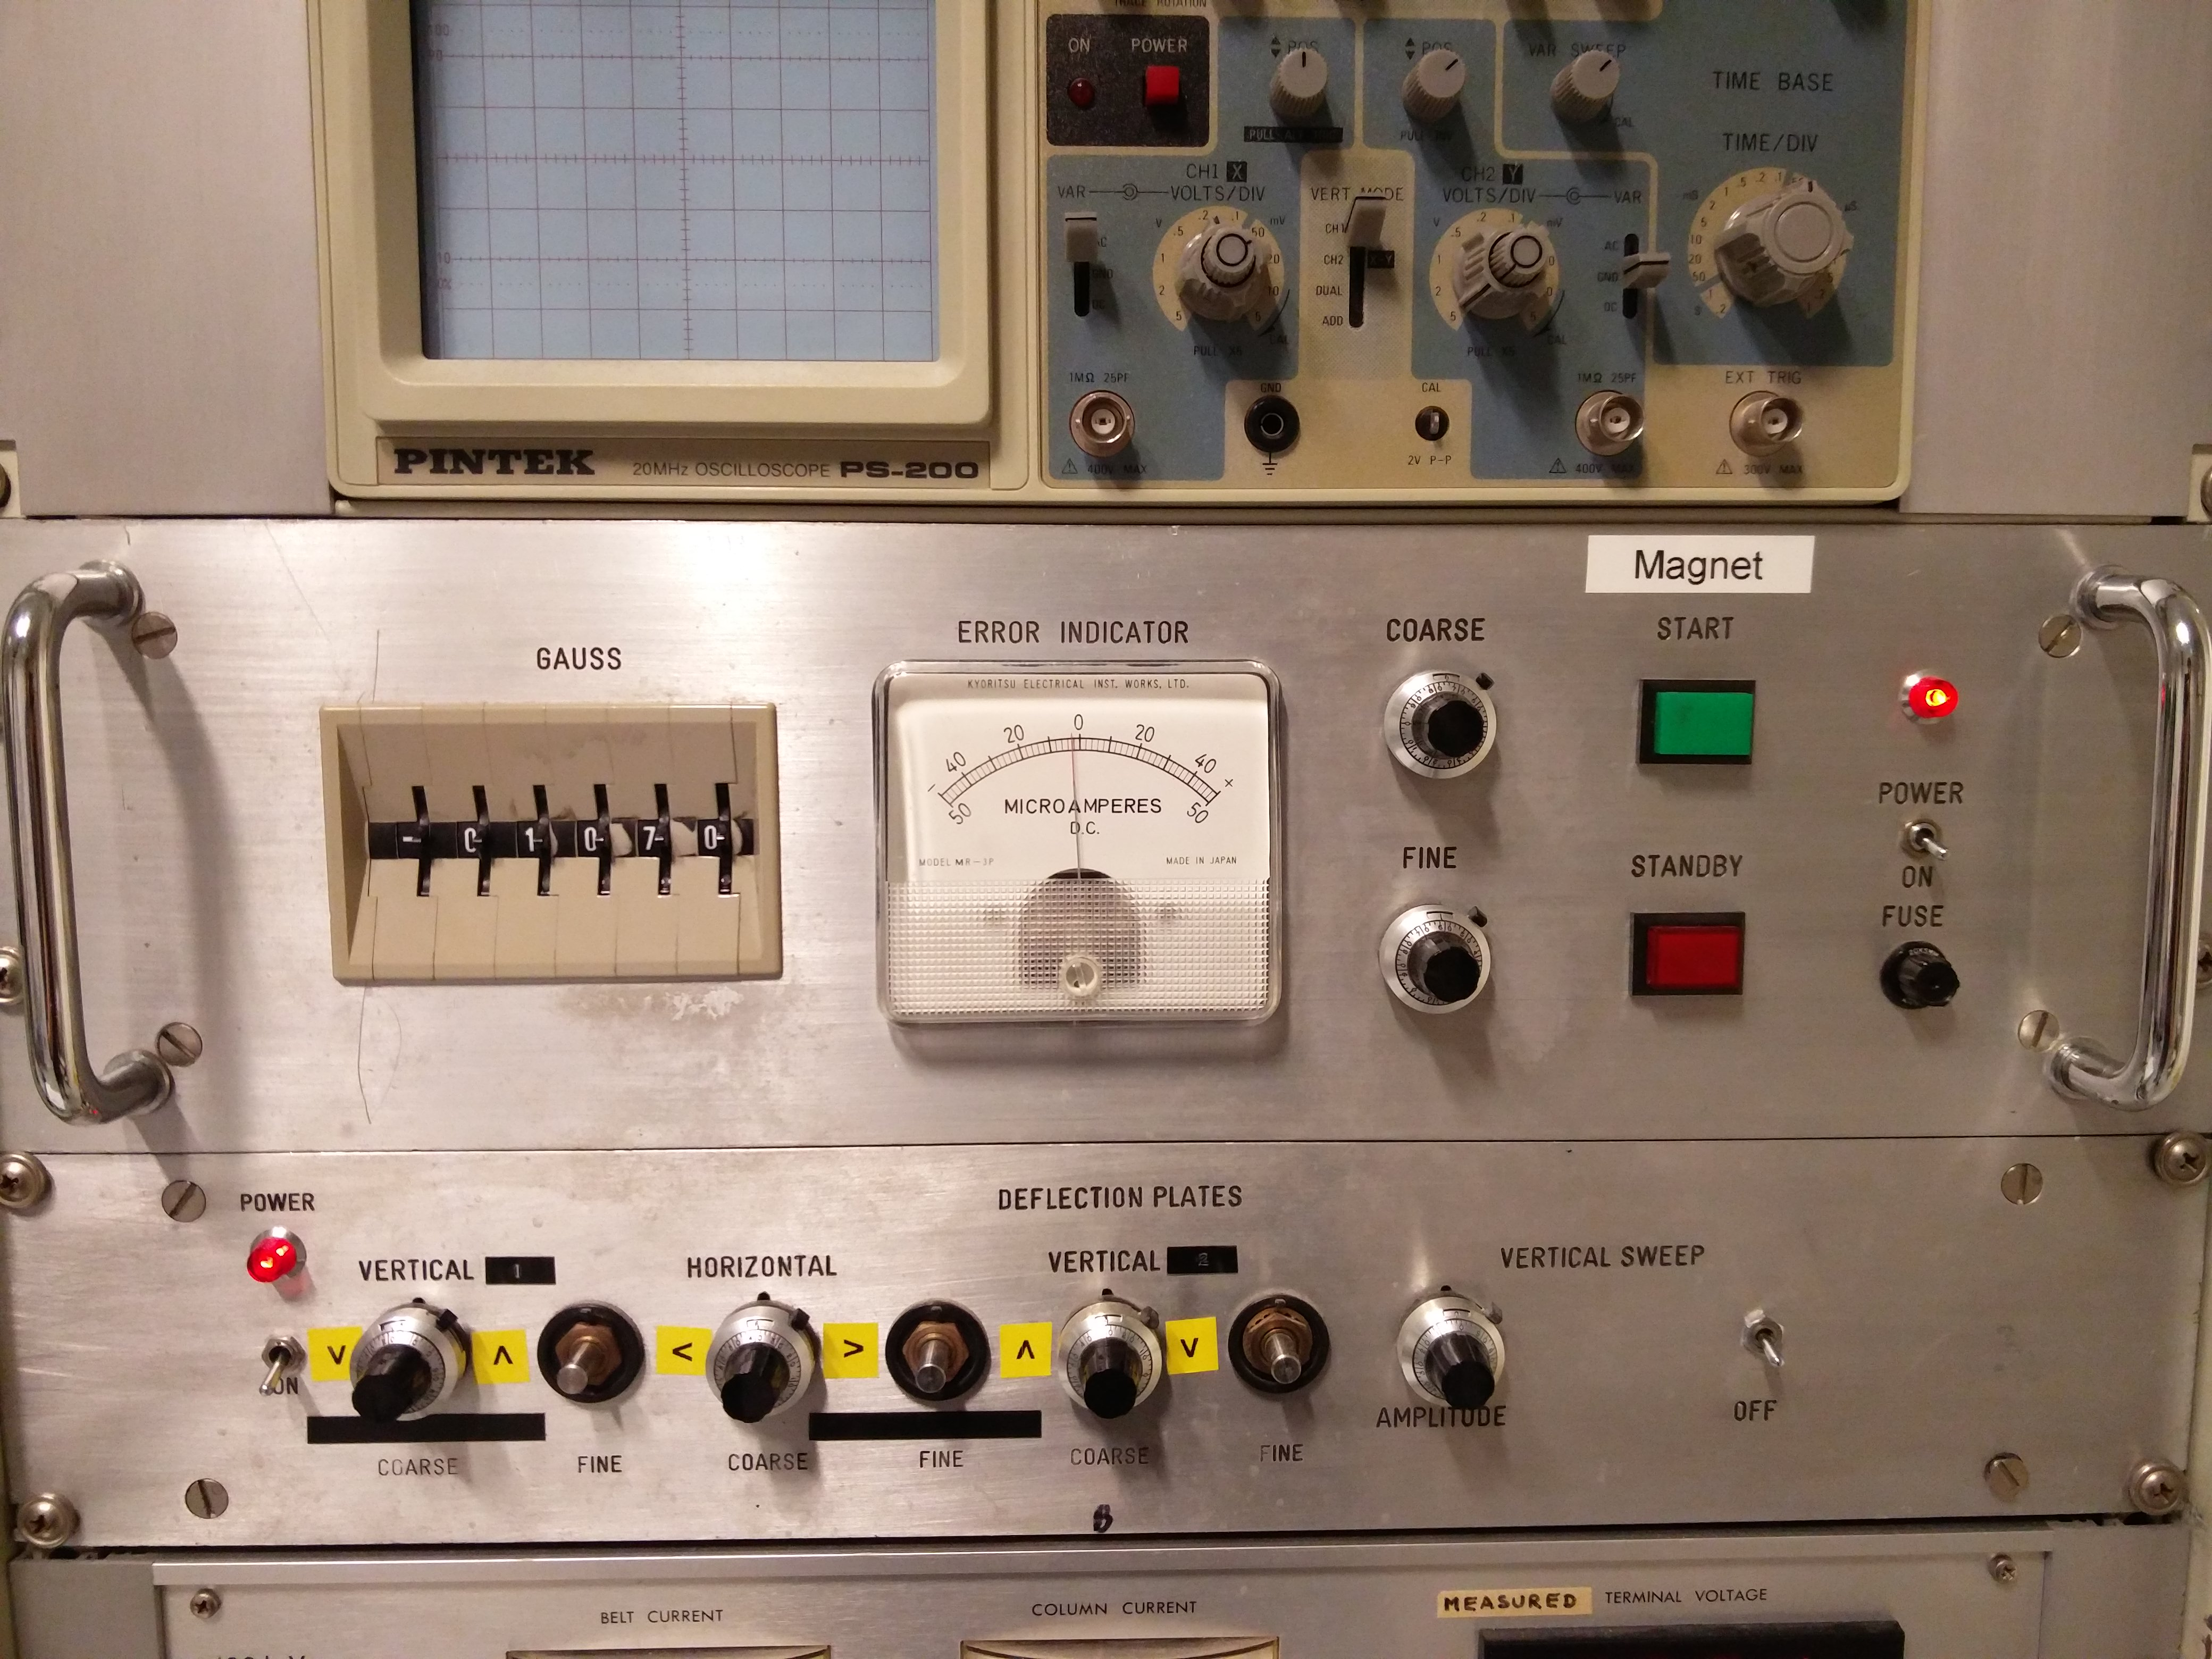
\includegraphics[trim={0, 30cm, 0, 30cm}, clip, width=0.99\columnwidth]{process3}
\caption{terminal voltage}
\label{fig_process3}
\end{figure}

\begin{figure}[h]
\centering
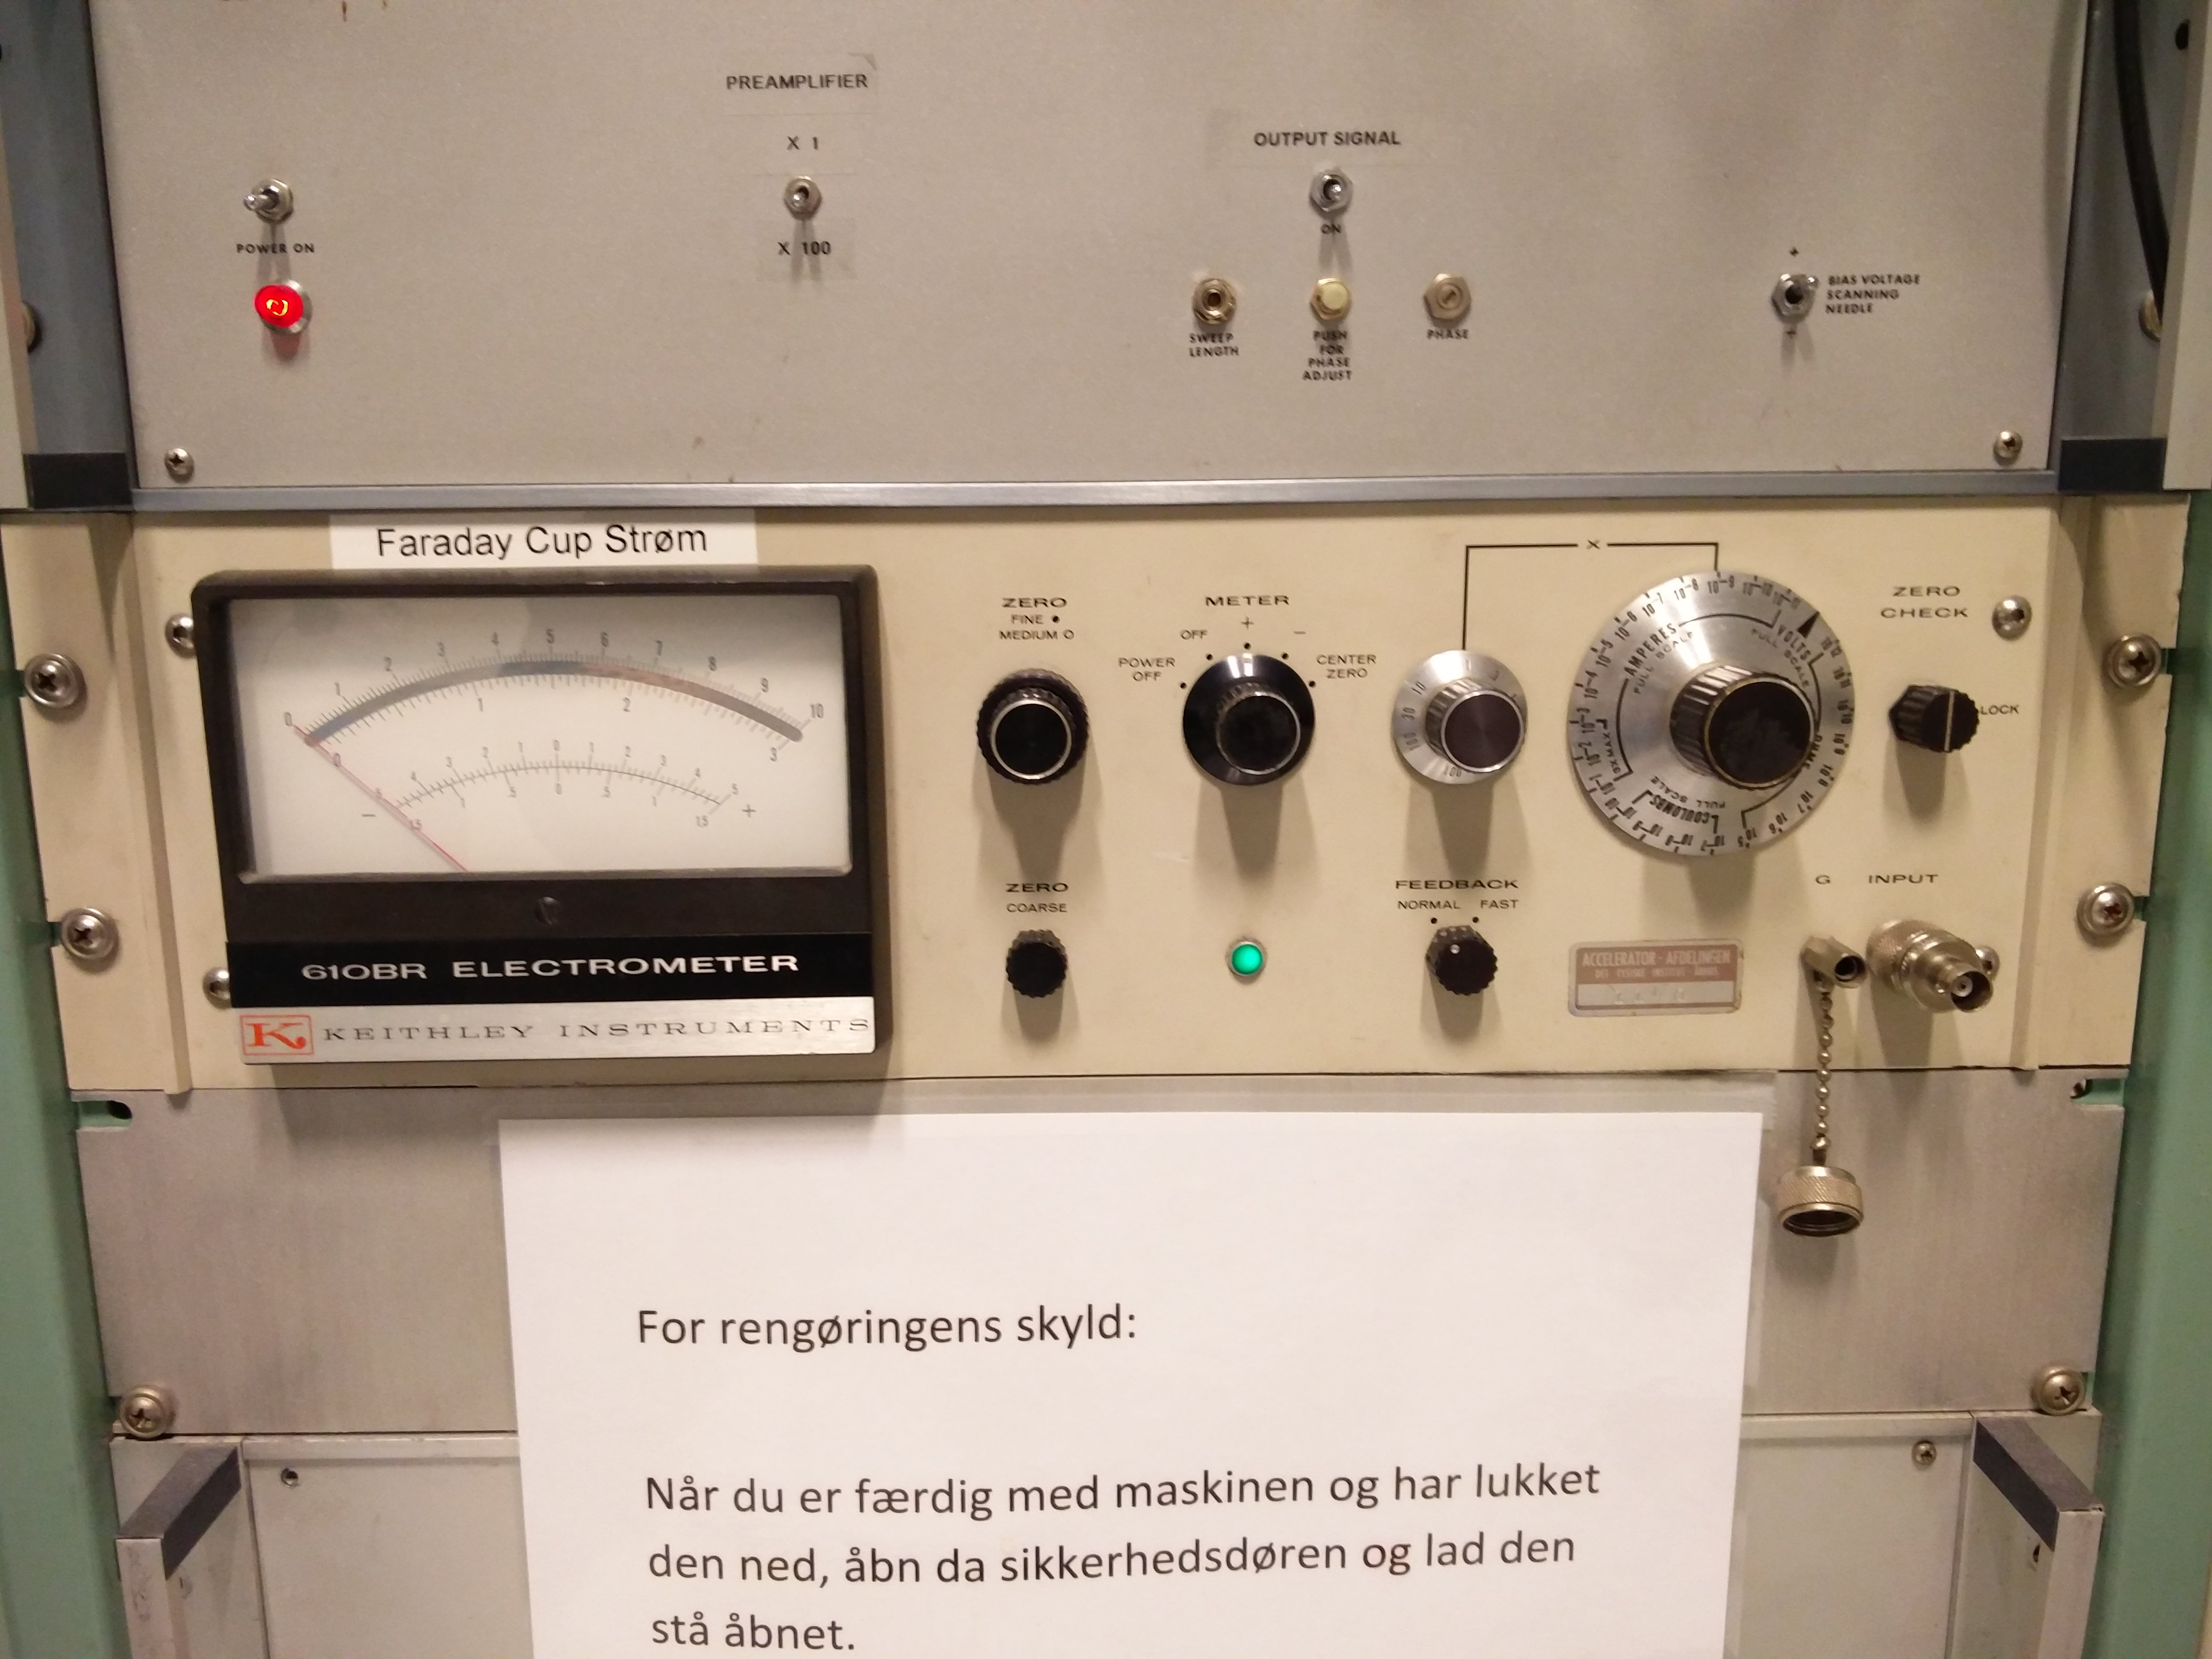
\includegraphics[trim={0, 35cm, 0, 30cm}, clip, width=0.99\columnwidth]{process4}
\caption{terminal voltage}
\label{fig_process4}
\end{figure}

When signal is good, set the voltage supply to ... 
\begin{figure}[h]
\centering
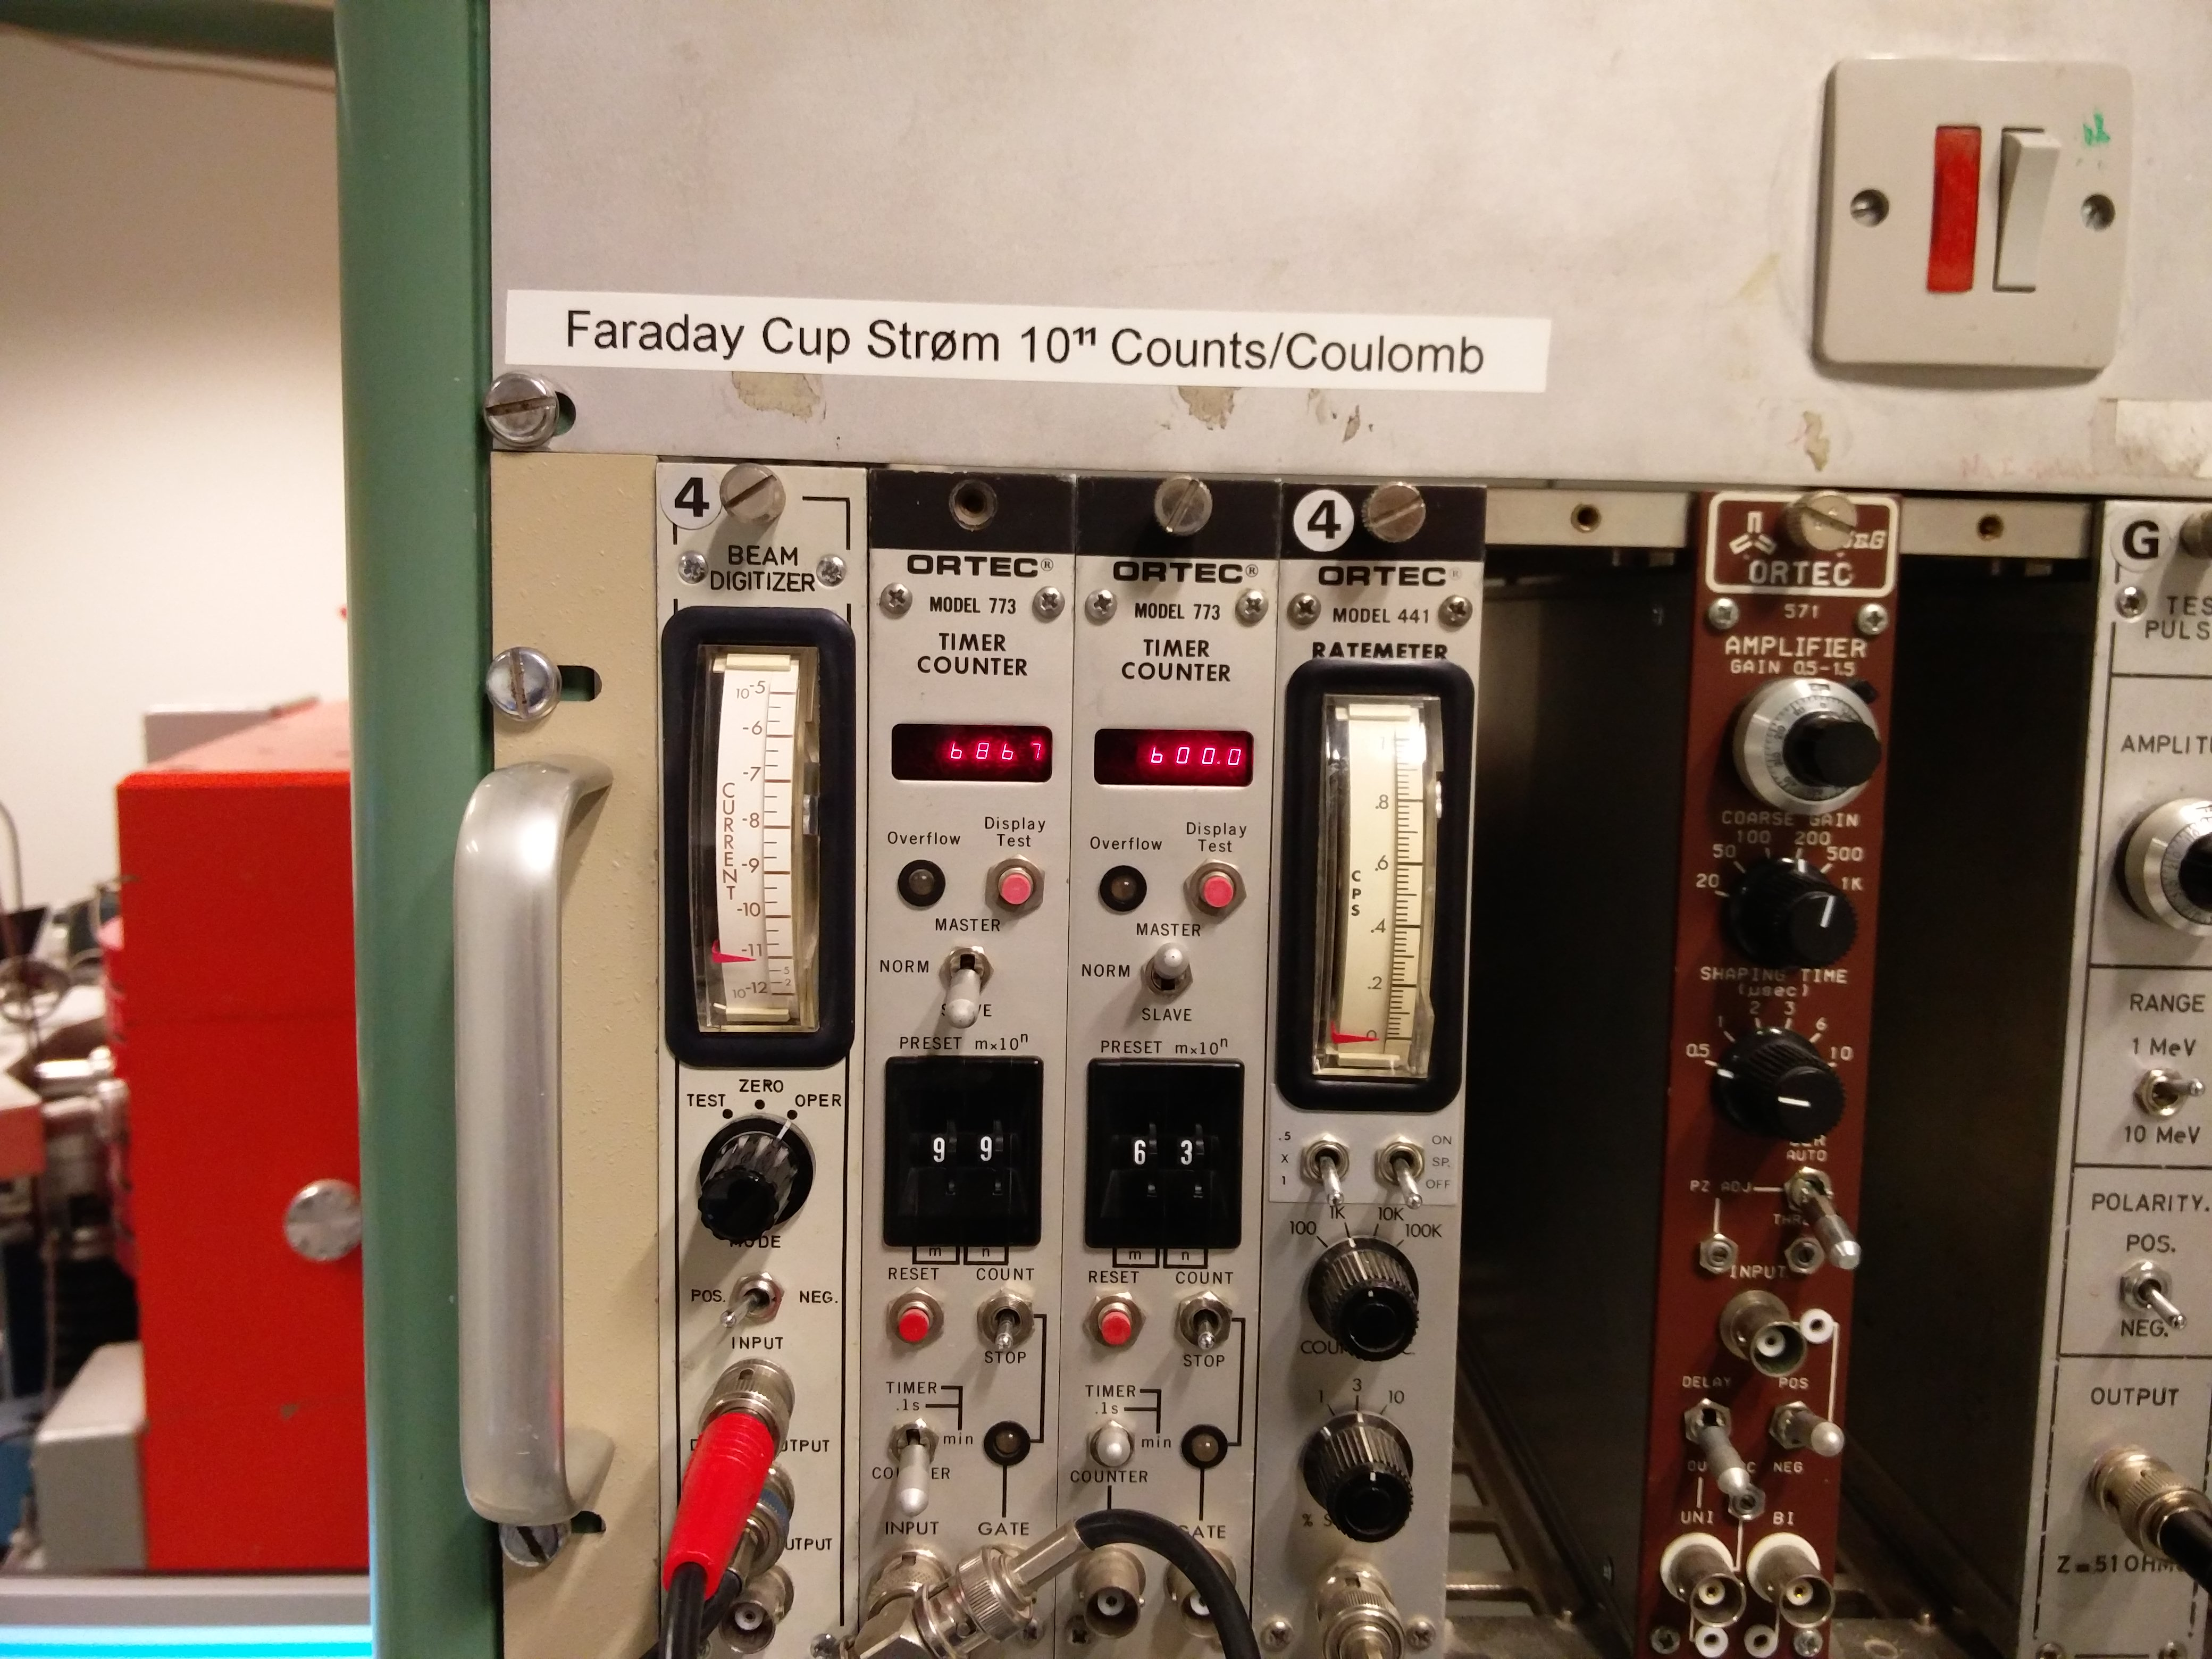
\includegraphics[trim={25cm, 0, 0, 15cm}, clip, width=0.99\columnwidth]{process5}
\caption{process5}
\label{fig_process5}
\end{figure}








\section{Angular dependency of the Rutherford cross section}
The Rutherford differential cross section \parencite[p. 16]{noteBB} is given by
\begin{align}\label{eq:cross}
    {\left( \diff[d]{\sigma}{\Omega} \right)}_|Rutherford| =
    {\left(\frac{Z_1Z_2 e^2}{4E_{\infty}} \right)}^2
    \frac{1}{{{\sin}^4(\frac{\theta}{2})}},
\end{align}
where $Z$ is the proton number of each interacting particle, $E_{\infty}$ is
the asymptotic energy, and $\theta$ is the scattering angle. If the energy is
in units of $\si{\mega\electronvolt}$, this differential cross section will be in units
of $\si{\milli\barn\per\steradian}$.\\
This formula neglects the recoil energy of the target. 

As mentioned earlier, the target has two layers, and thus the incomming beam of
ions can scatter on both gold and carbon. 

However, as the Rutherford scattering is a coulomb interaction and $Z_|Au| >
Z_|C|$, the Rutherford differential cross section for gold is greater than for carbon at any given angle. Hence we would expect the gold layer to scatter more particles at higher angles compared to carbon. Due to the same inequality of the nuclei number gold will also have a lower recoil energy, and thus from conservation of energy the particles scattered on gold will have a higher energy - bin number - than carbon.
%Furthermore, from the calibration it is found that the channel numbers are directly proportional to the meassured energies of the scattered particles. Combined with the fact that gold has a higher nuclei number than carbon and thus a lower recoil energy, we will expect the particles scattered on gold will have a higher energy than those of carbon from conservation of energy.

%From the calibration it is found that the channel number is directly proportional to the energy of the scattered particles. Combined with the fact, that gold has a higher mass number, and thus a lower recoil energy, it is expected that the particles scattered on the gold layer will have a higher energy, due to conservation of energy.

%% %%

To test the angular dependency of the Rutherford differential cross section,
the Silicon detector was set at a variable angle. At each angle the total
number of incomming particles and scattered particles were measured.\\

A Faraday cup was used to meassure the amount of non-scattered particles. 
Since this number is far greater than the amount of scattered particles, the
number of incomming particles can be assumed to be the number of detected
particles within the Faraday cup.\\

The number of any detected events in both the Faraday cup and the Silicon
detector follows a Poisson distribution, and thus the statistical uncertainty
goes as the square root of the total number of detected events.\\

The counted events from the Faraday cup can be read off the collector. 
The collector was set to relate $10^{11}$ counts per coulomb, and as there are
$6,24150913\ \cdot10^{18}$ elementary
charges per coulomb, we can relate the count number to an amount of detected
protons, $N$. Due to the beampipe, a factor of one half is also
necesarry.\footnote{Hans Fynbo, course responsible, mentioned this factor,
    which surprisingly fit well into our calculations.}

The relation between the number of incoming, $N$, and scattered particles, $dN$, is
\begin{equation}\label{eq:dN}
    \mathrm{d}N = N n_|tar| \mathrm{d}x \mathrm{d}\Omega,
    \diff[d]{\sigma(\theta,\phi)}{\Omega}.
\end{equation}
\parencite[eq. 14.42, p. 582]{taylor} where $n_|tar|$ and $\mathrm{d}x$ is the
nuclei density of the target thickness of the target respectivly, and
$\mathrm{d}\Omega$ is the small solid angle through which the scattered
particles emerge.

As previously mentioned  the two layered target will result in a double
scattered profile, thus a fit is expected to follow a double gaussian
distribution. Asuming a linear combination of the two gaussians one can
describe the count distribution \cref{fig_doublegauss}.\\
\begin{figure}[h]
\centering
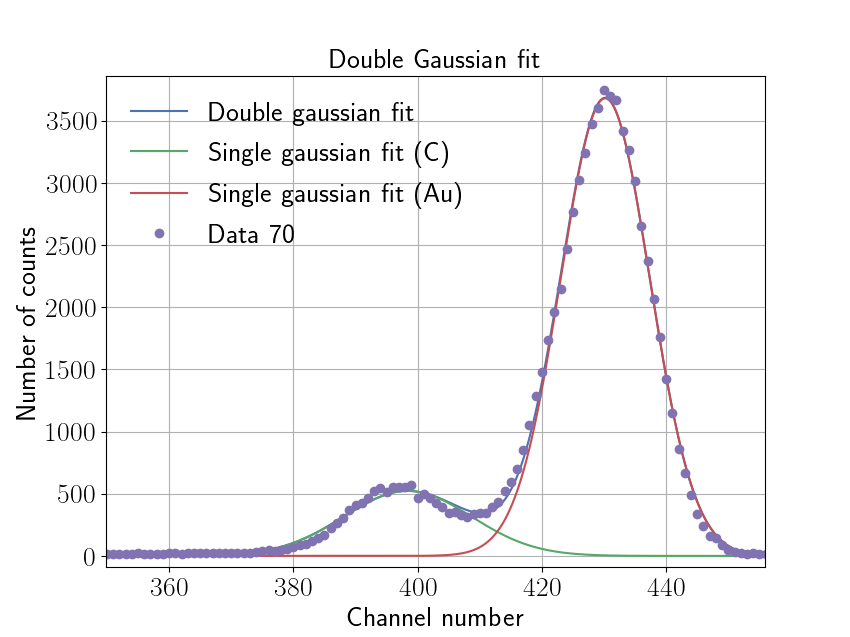
\includegraphics[width=0.99\columnwidth]{Data_70}
\caption{A double gaussian fit at a detector angle of $70$ degrees.}
\label{fig_doublegauss}
\end{figure}
Through a double gaussian fit we can distinguish between the scattered particles of gold and carbon, and determine their mean channel number corresponding to their energy.  \\
Fitting a double gaussian, one gather six parameters; amplitude, centroid and standard deviation
of both gaussians.  \\
%Notice in figure \ref{fig_angular_dependency} that the gaussian of greatest amplitude corresponds to gold, which
%is in agreement with the relative sizes of the two atoms. . Thus the recoil energy of gold is negligible compared to that of carbon.\\
Each gaussian term was used to determine the total count number by summing over
all channels, in order to obtain $\mathrm{d}N$ for particles scattered of gold
and carbon respectively.\\
%
From \cref{eq:dN} the differential cross section for each detector angle is
then calculated and compared to the expected differential cross section
\cref{eq:cross}.\\
\begin{figure}[h]
	\centering
		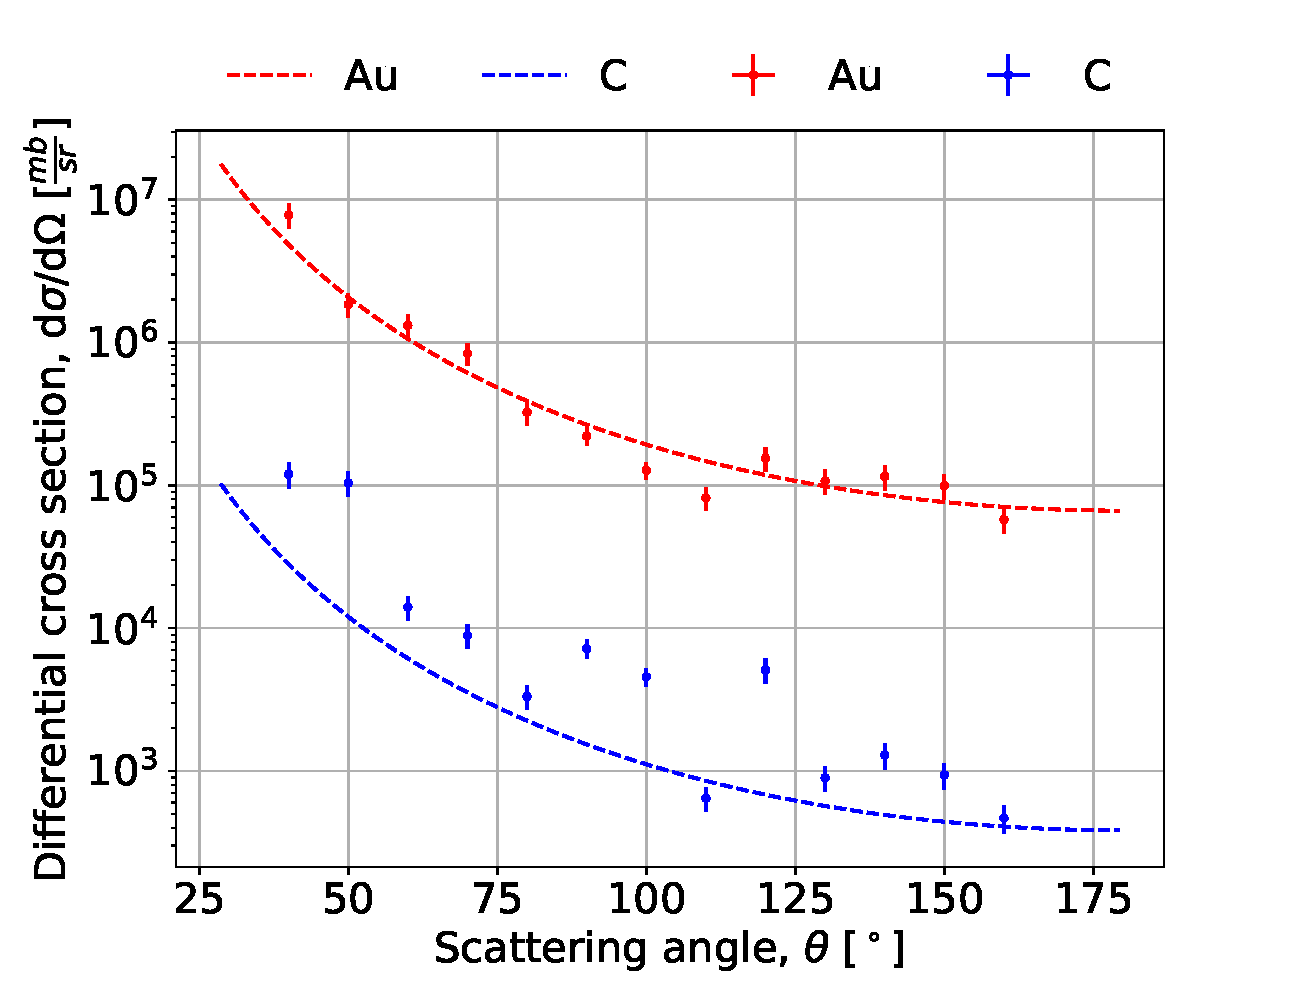
\includegraphics[width=0.45\textwidth]{Differential_cross_section.eps}
	\caption{The differential crossection  of carbon and gold as a function of the scattering angle. The dashed line represents the theoretical values.}
	\label{fig:Differential_cross_section}
\end{figure}
The data and the theoretical derived differential cross section have the same
characteristics though it seems as if all data for carbon is shifted to higher
values than what is expected by the theory.

The theoretical determined values are based on \cref{eq:cross}, which is under the assumption of a classical regime governt by the Sommerfeld criterion \parencite[p. 14]{noteBB}.
\begin{align}\label{eq:som}
\eta_|S|=0.16\cdot Z_1Z_2\sqrt{\frac{A_|proj|}{E_|lab|[\si{\mega\electronvolt}]}}\gg 1
\end{align}
For gold and carbon the values of the parameter is $\eta_|S|\sim 300$ and
$\eta_|S|\sim 6$ respectivly. It is interesting that the values for gold and carbon are in the order of $10^2$. Which could influence our theoretical assumptions for carbon. 

\section{Angular dependency of the proton energy}
From the double gaussian one obtains two centroids; one for each target layer.
These can be converted to the equivalent energies as described in the
calibration. Plotting the energy as a function of the detector angle
\cref{fig_energy}, it can be seen that the carbon layer radically changes
energies.
\begin{figure}[h!]
\centering
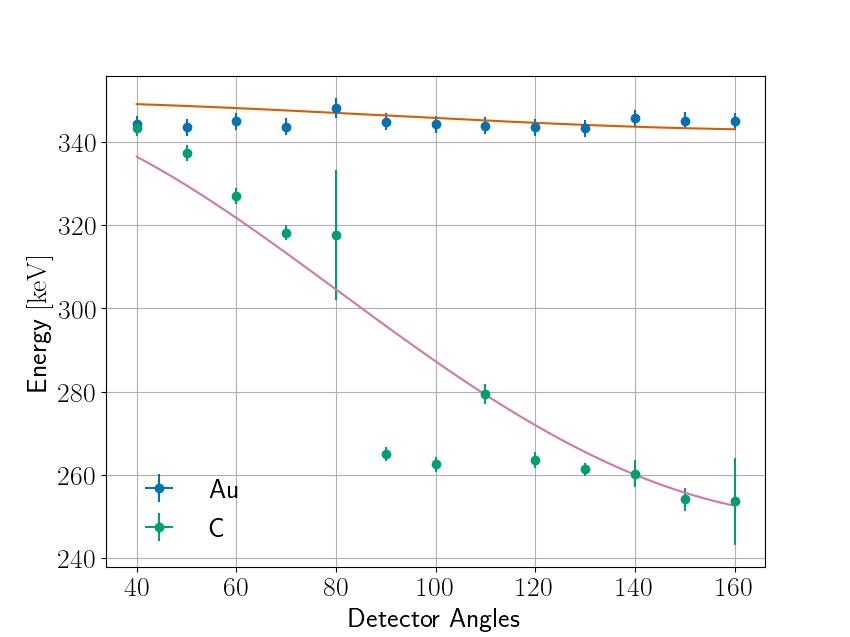
\includegraphics[width=0.99\columnwidth]{fig_energy}
\caption{Energies of Carbon and Gold scattered compared to theoretical
function.}
\label{fig_energy}
\end{figure}

On the otherhand gold is nearly constant. This is what is expected, as carbon
has a much higher recoil. Including the theoretical plot, as derived in
\cref{eq_5}, one can see that there exists some deviations from the expected
values. Especially at detector angles of $90$ and $100$ degrees.
A reason for this tendency, can be seen from \cref{fig_angular_dependency}. We
assume a linear combination of the gold and carbon distribution and thus fit a
double gaussian. Nonetheless, a small bump is seen between the carbon and gold
contributions. In a further analysis, one could fit a tripple gaussian and
identify the reason for this. The correction in bin number would shift it to
higher energy, which is just what would explain the lower energy than
expected.

Another interesting factor is how the two peaks change relative position as a
function of scattering, merging their gaussian distribution at low angles, \cref{fig_angular_dependency}. A complete overlap makes the seperation job more difficult, which explains the deviations at lower angles.




\section{Thickness of the target layers} 
Most of the particles pass directly through the target without scattering. However, a small amount do scatter. When particles pass through the first layer they loose energy. As a consequence, there will be a difference in the energy of the particles entering the first and the second layer. 

By comparing measurements of scattering on the target with gold layer facing the beam and the carbon layer facing the beam, the distributions for scattering on carbon and gold are observed at different energies \cref{fig_sketch_thickness}. 

\begin{figure}[h]
\centering
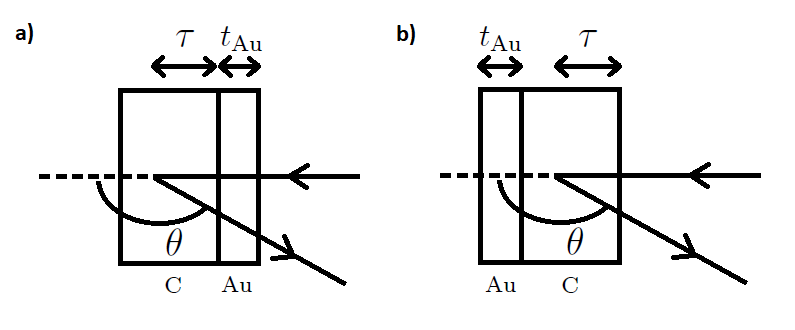
\includegraphics[width=0.99\columnwidth]{tykkelse.png}
\caption{Sketch of how to determine thickness of the target carbon layer from the energy difference between: a) gold layer facing the beam and b) carbon layer facing the beam.}
\label{fig_sketch_thickness}
\end{figure}

%The energies of the scattered protons is due to the ratio between the mass of the protons and the mass of the target. 
The energy differences are proportional to the thickness of target layers. To determine the thickness of the gold layer we consider what happens to the energy in the two following situations. In situation a) gold is facing the beam, and the final energy $E_{f,a}$ is given as the initial energy minus the energy lost due to the particles; passing through the gold layer, passing through part of the carbon layer, scattering on carbon, and passing through carbon and gold again on the way out, i.e.
\begin{align}
E_{f,a} &= f_\mathrm{C} \left[ E_i - \int_0^{t_{\mathrm{Au}}}{\left(\frac{dE}{dx}\right)_{\mathrm{Au}}dx} \right. \nonumber 
\\ &- \left. \int_0^{\tau}{\left(\frac{dE}{dx}\right)_{\mathrm{C}}dx} \right] \nonumber
\\ &- \int_0^{\frac{\tau}{\cos(\pi-\theta)}}{\left(\frac{dE}{dx}\right)_{\mathrm{C}}dx} \nonumber
\\ &- \int_0^{\frac{t_\mathrm{Au}}{\cos(\pi-\theta)}}{\left(\frac{dE}{dx}\right)_{\mathrm{Au}}dx}, 
\end{align}
where $f_\mathrm{C}$ is the function giving the relation between the incoming energy and the particle energy after scattering on gold in equation (6), $t_\mathrm{Au}$ is the thickness of the carbon layer and
$\left(\frac{dE}{dx}\right)_\mathrm{C}$ and $\left(\frac{dE}{dx}\right)_\mathrm{Au}$ is the stopping power of carbon and gold, respectively. With an initial hydrogen energy of $\SI{350}{\kilo\electronvolt}$ the
stopping power of carbon and gold are found to be $8.5$ and $34 \,
\si{\electronvolt}/(10^{15}$ atoms/$\si{\centi\metre}^2$), respectively. The
values were read off a table next to the laboratory equipment.

In situation b) carbon is facing the beam, and the final energy is given as the initial energy minus the energy lost due to the particles; passing through part the carbon layer, scattering on carbon, and passing through the carbon layer again on the way out. 
\begin{align}
E_{f,b} &= f_\mathrm{C} \left[ E_i - \int_0^{\tau}{\left(\frac{dE}{dx}\right)_{\mathrm{C}}dx} \right] \nonumber 
\\ &- \int_0^{\frac{\tau}{\cos(\pi-\theta)}}{\left(\frac{dE}{dx}\right)_{\mathrm{C}}dx}, 
\end{align}

The energy difference between the peak positions of carbon is found as the difference between the two situations;
\begin{align}
\Delta E_\mathrm{C} &= f_\mathrm{C} \int_0^{t_{\mathrm{Au}}}{\left(\frac{dE}{dx}\right)_{\mathrm{Au}}dx} \nonumber
\\ &+ \int_0^{\frac{t_\mathrm{Au}}{\cos(\pi-\theta)}}{\left(\frac{dE}{dx}\right)_{\mathrm{Au}}dx} \nonumber
\\ &= f_\mathrm{C} \cdot t_{\mathrm{Au}} \left( \frac{dE}{dx}\right)_{\mathrm{Au}} \nonumber
\\ &+ \frac{t_{\mathrm{Au}}}{\cos(\pi-\theta)} \left(\frac{dE}{dx}\right)_{\mathrm{Au}}
\end{align}
Thus, the thickness of the gold layer is
\begin{align}
t_{\mathrm{Au}} = \frac{\Delta E_\mathrm{C}}{ \left( f_\mathrm{C} + \frac{1}{\cos(\pi-\theta)} \right) \left( \frac{dE}{dx} \right)_{\mathrm{Au}} }
\end{align}
The thickness of the carbon layer is found using the same approach. 

\begin{table}[h]
\centering
\caption{Thickness of the target layers determined from change in energy.}
\begin{tabular}{CC}
\toprule
\multicolumn{2}{c}{Target layer thickness}\\
\midrule
\mathrm{C} & 1510 \pm 30 \; \AA \\
\mathrm{Au} & 250 \pm 25 \; \AA \\
\bottomrule
\end{tabular}

\label{tab_thickness}
\end{table}

%\begin{equation}
%\Delta E_{Au} = t_C \left(\frac{dE}{dx}\right)_C \left(1 - f_E(\theta) + %\frac{1}{\cos(\pi-\theta)} \right),
%\end{equation}



\begin{figure}[t]
\centering
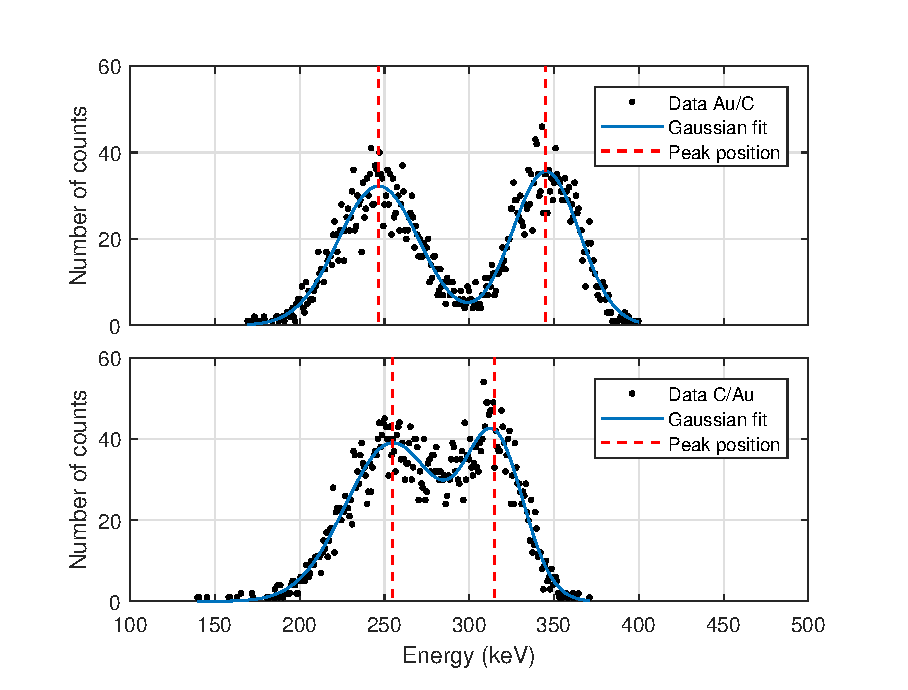
\includegraphics[width=0.99\columnwidth]{Dterminethicknessplot.eps}
\caption{Thickness of target layers determined from change in energy. Upper: gold layer facing the beam. Lower: carbon layer facing the beam.}
\label{fig_thickness}
\end{figure}

The scattering angle for thickness determination was chosen such that the distributions overlap as little as possible while still having sufficient number of counts for the case of gold facing the beam. However, significant overlap of the distributions is observed when turning the target 180 $\si{degrees}$ to situation b) where the carbon layer faces the beam. As discussed previously, overlap of distributions as well as low number of counts makes fitting two Gaussian functions difficult and thus affects the uncertainties for the determined fitting parameters.  In addition, the energy change for the carbon peak is very small, which complicates the determination of the precise thickness of the gold layer.









\section{Discussion}

\subsection{The experimental setup}
The Van de Graaf accelerator provide an enormous advantage over the
Cockcroft-Walton accelerator as the terminal voltage on a Van de Graaf is
extreemely stable and does not ripple as the later does. This is very important
when desired to measure reaction cross sections. Nonetheless, the Van de Graaf
accelerator has a low current output in the $\si{\micro\ampere}$ range compared
with the Cockcroft-Walton $\si{\milli\ampere}$. Nevertheless, this is quite
sufficient for nuclear reaction experiments, and thus our chosen accelerator is
the workhorse of low-energy nuclear structure physics.

To improve the potential drop across the accelerator:

Vacuum, so the limit of electrical breakdown (sparking) of 

To reduce breakdown and sparking, the generator is enclosed in a pressure tank
containing an insulating gas.
Capacitance (geometrical size)
\cite{krane}

\subsection{Rutherford experiment}
From 

Target dependency of the Rutherford cross section
Nuclear reactions of protons with boron.


\section{Conclusion}
During the experiment the Rutherford scattering has been examined. A relation between the differential cross section have been determined and compared with the theory assuming that the Summerfeld criterion is fulfilled. 


The classical Rutherford scattering of low energy hydrogenic ions, $H^+$ and $H_2^+$ on a double layered target of $\SI{20}{\angstrom}$ gold and $\SI{200}{\angstrom}$ carbon have been examined. Especially the angular dependency of the scattered particles was investigated. 


There is a clear relation between the fit of the data counts and the deviation of the theoretical expected energies.  

Accordingly, two gaussians; one for carbon and another for gold, was fitted. For small angles the two gaussians merged, making the estimation of the centroid more difficult. For larger angles, this problem is avoided. Another problem occur. We see a small bump in between the carbon and gold gaussians. Thus our assumption of a double gaussian is bad. This could be dodged had we fitted a tripple gaussian, which might shift the the carbon centroid towards higher bins and thus a higher energy. 



We assumed a linear combination of the two gaussian distributions. Nonetheless, this might have lead to 


\clearpage
\printbibliography[heading=subbibliography]{}
\nocite{*}
\end{document}

